
\documentclass[10pt]{article} % For LaTeX2e
\usepackage{tmlr}
% If accepted, instead use the following line for the camera-ready submission:
%\usepackage[accepted]{tmlr}
% To de-anonymize and remove mentions to TMLR (for example for posting to preprint servers), instead use the following:
%\usepackage{tmlr}

% Optional math commands (vendored).
%%%%% NEW MATH DEFINITIONS %%%%%

\usepackage{amsmath,amsfonts,bm}

% Mark sections of captions for referring to divisions of figures
\newcommand{\figleft}{{\em (Left)}}
\newcommand{\figcenter}{{\em (Center)}}
\newcommand{\figright}{{\em (Right)}}
\newcommand{\figtop}{{\em (Top)}}
\newcommand{\figbottom}{{\em (Bottom)}}
\newcommand{\captiona}{{\em (a)}}
\newcommand{\captionb}{{\em (b)}}
\newcommand{\captionc}{{\em (c)}}
\newcommand{\captiond}{{\em (d)}}

% Highlight a newly defined term
\newcommand{\newterm}[1]{{\bf #1}}


% Figure reference, lower-case.
\def\figref#1{figure~\ref{#1}}
% Figure reference, capital. For start of sentence
\def\Figref#1{Figure~\ref{#1}}
\def\twofigref#1#2{figures \ref{#1} and \ref{#2}}
\def\quadfigref#1#2#3#4{figures \ref{#1}, \ref{#2}, \ref{#3} and \ref{#4}}
% Section reference, lower-case.
\def\secref#1{section~\ref{#1}}
% Section reference, capital.
\def\Secref#1{Section~\ref{#1}}
% Reference to two sections.
\def\twosecrefs#1#2{sections \ref{#1} and \ref{#2}}
% Reference to three sections.
\def\secrefs#1#2#3{sections \ref{#1}, \ref{#2} and \ref{#3}}
% Reference to an equation, lower-case.
\def\eqref#1{equation~\ref{#1}}
% Reference to an equation, upper case
\def\Eqref#1{Equation~\ref{#1}}
% A raw reference to an equation---avoid using if possible
\def\plaineqref#1{\ref{#1}}
% Reference to a chapter, lower-case.
\def\chapref#1{chapter~\ref{#1}}
% Reference to an equation, upper case.
\def\Chapref#1{Chapter~\ref{#1}}
% Reference to a range of chapters
\def\rangechapref#1#2{chapters\ref{#1}--\ref{#2}}
% Reference to an algorithm, lower-case.
\def\algref#1{algorithm~\ref{#1}}
% Reference to an algorithm, upper case.
\def\Algref#1{Algorithm~\ref{#1}}
\def\twoalgref#1#2{algorithms \ref{#1} and \ref{#2}}
\def\Twoalgref#1#2{Algorithms \ref{#1} and \ref{#2}}
% Reference to a part, lower case
\def\partref#1{part~\ref{#1}}
% Reference to a part, upper case
\def\Partref#1{Part~\ref{#1}}
\def\twopartref#1#2{parts \ref{#1} and \ref{#2}}

\def\ceil#1{\lceil #1 \rceil}
\def\floor#1{\lfloor #1 \rfloor}
\def\1{\bm{1}}
\newcommand{\train}{\mathcal{D}}
\newcommand{\valid}{\mathcal{D_{\mathrm{valid}}}}
\newcommand{\test}{\mathcal{D_{\mathrm{test}}}}

\def\eps{{\epsilon}}


% Random variables
\def\reta{{\textnormal{$\eta$}}}
\def\ra{{\textnormal{a}}}
\def\rb{{\textnormal{b}}}
\def\rc{{\textnormal{c}}}
\def\rd{{\textnormal{d}}}
\def\re{{\textnormal{e}}}
\def\rf{{\textnormal{f}}}
\def\rg{{\textnormal{g}}}
\def\rh{{\textnormal{h}}}
\def\ri{{\textnormal{i}}}
\def\rj{{\textnormal{j}}}
\def\rk{{\textnormal{k}}}
\def\rl{{\textnormal{l}}}
% rm is already a command, just don't name any random variables m
\def\rn{{\textnormal{n}}}
\def\ro{{\textnormal{o}}}
\def\rp{{\textnormal{p}}}
\def\rq{{\textnormal{q}}}
\def\rr{{\textnormal{r}}}
\def\rs{{\textnormal{s}}}
\def\rt{{\textnormal{t}}}
\def\ru{{\textnormal{u}}}
\def\rv{{\textnormal{v}}}
\def\rw{{\textnormal{w}}}
\def\rx{{\textnormal{x}}}
\def\ry{{\textnormal{y}}}
\def\rz{{\textnormal{z}}}

% Random vectors
\def\rvepsilon{{\mathbf{\epsilon}}}
\def\rvtheta{{\mathbf{\theta}}}
\def\rva{{\mathbf{a}}}
\def\rvb{{\mathbf{b}}}
\def\rvc{{\mathbf{c}}}
\def\rvd{{\mathbf{d}}}
\def\rve{{\mathbf{e}}}
\def\rvf{{\mathbf{f}}}
\def\rvg{{\mathbf{g}}}
\def\rvh{{\mathbf{h}}}
\def\rvu{{\mathbf{i}}}
\def\rvj{{\mathbf{j}}}
\def\rvk{{\mathbf{k}}}
\def\rvl{{\mathbf{l}}}
\def\rvm{{\mathbf{m}}}
\def\rvn{{\mathbf{n}}}
\def\rvo{{\mathbf{o}}}
\def\rvp{{\mathbf{p}}}
\def\rvq{{\mathbf{q}}}
\def\rvr{{\mathbf{r}}}
\def\rvs{{\mathbf{s}}}
\def\rvt{{\mathbf{t}}}
\def\rvu{{\mathbf{u}}}
\def\rvv{{\mathbf{v}}}
\def\rvw{{\mathbf{w}}}
\def\rvx{{\mathbf{x}}}
\def\rvy{{\mathbf{y}}}
\def\rvz{{\mathbf{z}}}

% Elements of random vectors
\def\erva{{\textnormal{a}}}
\def\ervb{{\textnormal{b}}}
\def\ervc{{\textnormal{c}}}
\def\ervd{{\textnormal{d}}}
\def\erve{{\textnormal{e}}}
\def\ervf{{\textnormal{f}}}
\def\ervg{{\textnormal{g}}}
\def\ervh{{\textnormal{h}}}
\def\ervi{{\textnormal{i}}}
\def\ervj{{\textnormal{j}}}
\def\ervk{{\textnormal{k}}}
\def\ervl{{\textnormal{l}}}
\def\ervm{{\textnormal{m}}}
\def\ervn{{\textnormal{n}}}
\def\ervo{{\textnormal{o}}}
\def\ervp{{\textnormal{p}}}
\def\ervq{{\textnormal{q}}}
\def\ervr{{\textnormal{r}}}
\def\ervs{{\textnormal{s}}}
\def\ervt{{\textnormal{t}}}
\def\ervu{{\textnormal{u}}}
\def\ervv{{\textnormal{v}}}
\def\ervw{{\textnormal{w}}}
\def\ervx{{\textnormal{x}}}
\def\ervy{{\textnormal{y}}}
\def\ervz{{\textnormal{z}}}

% Random matrices
\def\rmA{{\mathbf{A}}}
\def\rmB{{\mathbf{B}}}
\def\rmC{{\mathbf{C}}}
\def\rmD{{\mathbf{D}}}
\def\rmE{{\mathbf{E}}}
\def\rmF{{\mathbf{F}}}
\def\rmG{{\mathbf{G}}}
\def\rmH{{\mathbf{H}}}
\def\rmI{{\mathbf{I}}}
\def\rmJ{{\mathbf{J}}}
\def\rmK{{\mathbf{K}}}
\def\rmL{{\mathbf{L}}}
\def\rmM{{\mathbf{M}}}
\def\rmN{{\mathbf{N}}}
\def\rmO{{\mathbf{O}}}
\def\rmP{{\mathbf{P}}}
\def\rmQ{{\mathbf{Q}}}
\def\rmR{{\mathbf{R}}}
\def\rmS{{\mathbf{S}}}
\def\rmT{{\mathbf{T}}}
\def\rmU{{\mathbf{U}}}
\def\rmV{{\mathbf{V}}}
\def\rmW{{\mathbf{W}}}
\def\rmX{{\mathbf{X}}}
\def\rmY{{\mathbf{Y}}}
\def\rmZ{{\mathbf{Z}}}

% Elements of random matrices
\def\ermA{{\textnormal{A}}}
\def\ermB{{\textnormal{B}}}
\def\ermC{{\textnormal{C}}}
\def\ermD{{\textnormal{D}}}
\def\ermE{{\textnormal{E}}}
\def\ermF{{\textnormal{F}}}
\def\ermG{{\textnormal{G}}}
\def\ermH{{\textnormal{H}}}
\def\ermI{{\textnormal{I}}}
\def\ermJ{{\textnormal{J}}}
\def\ermK{{\textnormal{K}}}
\def\ermL{{\textnormal{L}}}
\def\ermM{{\textnormal{M}}}
\def\ermN{{\textnormal{N}}}
\def\ermO{{\textnormal{O}}}
\def\ermP{{\textnormal{P}}}
\def\ermQ{{\textnormal{Q}}}
\def\ermR{{\textnormal{R}}}
\def\ermS{{\textnormal{S}}}
\def\ermT{{\textnormal{T}}}
\def\ermU{{\textnormal{U}}}
\def\ermV{{\textnormal{V}}}
\def\ermW{{\textnormal{W}}}
\def\ermX{{\textnormal{X}}}
\def\ermY{{\textnormal{Y}}}
\def\ermZ{{\textnormal{Z}}}

% Vectors
\def\vzero{{\bm{0}}}
\def\vone{{\bm{1}}}
\def\vmu{{\bm{\mu}}}
\def\vtheta{{\bm{\theta}}}
\def\va{{\bm{a}}}
\def\vb{{\bm{b}}}
\def\vc{{\bm{c}}}
\def\vd{{\bm{d}}}
\def\ve{{\bm{e}}}
\def\vf{{\bm{f}}}
\def\vg{{\bm{g}}}
\def\vh{{\bm{h}}}
\def\vi{{\bm{i}}}
\def\vj{{\bm{j}}}
\def\vk{{\bm{k}}}
\def\vl{{\bm{l}}}
\def\vm{{\bm{m}}}
\def\vn{{\bm{n}}}
\def\vo{{\bm{o}}}
\def\vp{{\bm{p}}}
\def\vq{{\bm{q}}}
\def\vr{{\bm{r}}}
\def\vs{{\bm{s}}}
\def\vt{{\bm{t}}}
\def\vu{{\bm{u}}}
\def\vv{{\bm{v}}}
\def\vw{{\bm{w}}}
\def\vx{{\bm{x}}}
\def\vy{{\bm{y}}}
\def\vz{{\bm{z}}}

% Elements of vectors
\def\evalpha{{\alpha}}
\def\evbeta{{\beta}}
\def\evepsilon{{\epsilon}}
\def\evlambda{{\lambda}}
\def\evomega{{\omega}}
\def\evmu{{\mu}}
\def\evpsi{{\psi}}
\def\evsigma{{\sigma}}
\def\evtheta{{\theta}}
\def\eva{{a}}
\def\evb{{b}}
\def\evc{{c}}
\def\evd{{d}}
\def\eve{{e}}
\def\evf{{f}}
\def\evg{{g}}
\def\evh{{h}}
\def\evi{{i}}
\def\evj{{j}}
\def\evk{{k}}
\def\evl{{l}}
\def\evm{{m}}
\def\evn{{n}}
\def\evo{{o}}
\def\evp{{p}}
\def\evq{{q}}
\def\evr{{r}}
\def\evs{{s}}
\def\evt{{t}}
\def\evu{{u}}
\def\evv{{v}}
\def\evw{{w}}
\def\evx{{x}}
\def\evy{{y}}
\def\evz{{z}}

% Matrix
\def\mA{{\bm{A}}}
\def\mB{{\bm{B}}}
\def\mC{{\bm{C}}}
\def\mD{{\bm{D}}}
\def\mE{{\bm{E}}}
\def\mF{{\bm{F}}}
\def\mG{{\bm{G}}}
\def\mH{{\bm{H}}}
\def\mI{{\bm{I}}}
\def\mJ{{\bm{J}}}
\def\mK{{\bm{K}}}
\def\mL{{\bm{L}}}
\def\mM{{\bm{M}}}
\def\mN{{\bm{N}}}
\def\mO{{\bm{O}}}
\def\mP{{\bm{P}}}
\def\mQ{{\bm{Q}}}
\def\mR{{\bm{R}}}
\def\mS{{\bm{S}}}
\def\mT{{\bm{T}}}
\def\mU{{\bm{U}}}
\def\mV{{\bm{V}}}
\def\mW{{\bm{W}}}
\def\mX{{\bm{X}}}
\def\mY{{\bm{Y}}}
\def\mZ{{\bm{Z}}}
\def\mBeta{{\bm{\beta}}}
\def\mPhi{{\bm{\Phi}}}
\def\mLambda{{\bm{\Lambda}}}
\def\mSigma{{\bm{\Sigma}}}

% Tensor
\DeclareMathAlphabet{\mathsfit}{\encodingdefault}{\sfdefault}{m}{sl}
\SetMathAlphabet{\mathsfit}{bold}{\encodingdefault}{\sfdefault}{bx}{n}
\newcommand{\tens}[1]{\bm{\mathsfit{#1}}}
\def\tA{{\tens{A}}}
\def\tB{{\tens{B}}}
\def\tC{{\tens{C}}}
\def\tD{{\tens{D}}}
\def\tE{{\tens{E}}}
\def\tF{{\tens{F}}}
\def\tG{{\tens{G}}}
\def\tH{{\tens{H}}}
\def\tI{{\tens{I}}}
\def\tJ{{\tens{J}}}
\def\tK{{\tens{K}}}
\def\tL{{\tens{L}}}
\def\tM{{\tens{M}}}
\def\tN{{\tens{N}}}
\def\tO{{\tens{O}}}
\def\tP{{\tens{P}}}
\def\tQ{{\tens{Q}}}
\def\tR{{\tens{R}}}
\def\tS{{\tens{S}}}
\def\tT{{\tens{T}}}
\def\tU{{\tens{U}}}
\def\tV{{\tens{V}}}
\def\tW{{\tens{W}}}
\def\tX{{\tens{X}}}
\def\tY{{\tens{Y}}}
\def\tZ{{\tens{Z}}}


% Graph
\def\gA{{\mathcal{A}}}
\def\gB{{\mathcal{B}}}
\def\gC{{\mathcal{C}}}
\def\gD{{\mathcal{D}}}
\def\gE{{\mathcal{E}}}
\def\gF{{\mathcal{F}}}
\def\gG{{\mathcal{G}}}
\def\gH{{\mathcal{H}}}
\def\gI{{\mathcal{I}}}
\def\gJ{{\mathcal{J}}}
\def\gK{{\mathcal{K}}}
\def\gL{{\mathcal{L}}}
\def\gM{{\mathcal{M}}}
\def\gN{{\mathcal{N}}}
\def\gO{{\mathcal{O}}}
\def\gP{{\mathcal{P}}}
\def\gQ{{\mathcal{Q}}}
\def\gR{{\mathcal{R}}}
\def\gS{{\mathcal{S}}}
\def\gT{{\mathcal{T}}}
\def\gU{{\mathcal{U}}}
\def\gV{{\mathcal{V}}}
\def\gW{{\mathcal{W}}}
\def\gX{{\mathcal{X}}}
\def\gY{{\mathcal{Y}}}
\def\gZ{{\mathcal{Z}}}

% Sets
\def\sA{{\mathbb{A}}}
\def\sB{{\mathbb{B}}}
\def\sC{{\mathbb{C}}}
\def\sD{{\mathbb{D}}}
% Don't use a set called E, because this would be the same as our symbol
% for expectation.
\def\sF{{\mathbb{F}}}
\def\sG{{\mathbb{G}}}
\def\sH{{\mathbb{H}}}
\def\sI{{\mathbb{I}}}
\def\sJ{{\mathbb{J}}}
\def\sK{{\mathbb{K}}}
\def\sL{{\mathbb{L}}}
\def\sM{{\mathbb{M}}}
\def\sN{{\mathbb{N}}}
\def\sO{{\mathbb{O}}}
\def\sP{{\mathbb{P}}}
\def\sQ{{\mathbb{Q}}}
\def\sR{{\mathbb{R}}}
\def\sS{{\mathbb{S}}}
\def\sT{{\mathbb{T}}}
\def\sU{{\mathbb{U}}}
\def\sV{{\mathbb{V}}}
\def\sW{{\mathbb{W}}}
\def\sX{{\mathbb{X}}}
\def\sY{{\mathbb{Y}}}
\def\sZ{{\mathbb{Z}}}

% Entries of a matrix
\def\emLambda{{\Lambda}}
\def\emA{{A}}
\def\emB{{B}}
\def\emC{{C}}
\def\emD{{D}}
\def\emE{{E}}
\def\emF{{F}}
\def\emG{{G}}
\def\emH{{H}}
\def\emI{{I}}
\def\emJ{{J}}
\def\emK{{K}}
\def\emL{{L}}
\def\emM{{M}}
\def\emN{{N}}
\def\emO{{O}}
\def\emP{{P}}
\def\emQ{{Q}}
\def\emR{{R}}
\def\emS{{S}}
\def\emT{{T}}
\def\emU{{U}}
\def\emV{{V}}
\def\emW{{W}}
\def\emX{{X}}
\def\emY{{Y}}
\def\emZ{{Z}}
\def\emSigma{{\Sigma}}

% entries of a tensor
% Same font as tensor, without \bm wrapper
\newcommand{\etens}[1]{\mathsfit{#1}}
\def\etLambda{{\etens{\Lambda}}}
\def\etA{{\etens{A}}}
\def\etB{{\etens{B}}}
\def\etC{{\etens{C}}}
\def\etD{{\etens{D}}}
\def\etE{{\etens{E}}}
\def\etF{{\etens{F}}}
\def\etG{{\etens{G}}}
\def\etH{{\etens{H}}}
\def\etI{{\etens{I}}}
\def\etJ{{\etens{J}}}
\def\etK{{\etens{K}}}
\def\etL{{\etens{L}}}
\def\etM{{\etens{M}}}
\def\etN{{\etens{N}}}
\def\etO{{\etens{O}}}
\def\etP{{\etens{P}}}
\def\etQ{{\etens{Q}}}
\def\etR{{\etens{R}}}
\def\etS{{\etens{S}}}
\def\etT{{\etens{T}}}
\def\etU{{\etens{U}}}
\def\etV{{\etens{V}}}
\def\etW{{\etens{W}}}
\def\etX{{\etens{X}}}
\def\etY{{\etens{Y}}}
\def\etZ{{\etens{Z}}}

% The true underlying data generating distribution
\newcommand{\pdata}{p_{\rm{data}}}
% The empirical distribution defined by the training set
\newcommand{\ptrain}{\hat{p}_{\rm{data}}}
\newcommand{\Ptrain}{\hat{P}_{\rm{data}}}
% The model distribution
\newcommand{\pmodel}{p_{\rm{model}}}
\newcommand{\Pmodel}{P_{\rm{model}}}
\newcommand{\ptildemodel}{\tilde{p}_{\rm{model}}}
% Stochastic autoencoder distributions
\newcommand{\pencode}{p_{\rm{encoder}}}
\newcommand{\pdecode}{p_{\rm{decoder}}}
\newcommand{\precons}{p_{\rm{reconstruct}}}

\newcommand{\laplace}{\mathrm{Laplace}} % Laplace distribution

\newcommand{\E}{\mathbb{E}}
\newcommand{\Ls}{\mathcal{L}}
\newcommand{\R}{\mathbb{R}}
\newcommand{\emp}{\tilde{p}}
\newcommand{\lr}{\alpha}
\newcommand{\reg}{\lambda}
\newcommand{\rect}{\mathrm{rectifier}}
\newcommand{\softmax}{\mathrm{softmax}}
\newcommand{\sigmoid}{\sigma}
\newcommand{\softplus}{\zeta}
\newcommand{\KL}{D_{\mathrm{KL}}}
\newcommand{\Var}{\mathrm{Var}}
\newcommand{\standarderror}{\mathrm{SE}}
\newcommand{\Cov}{\mathrm{Cov}}
% Wolfram Mathworld says $L^2$ is for function spaces and $\ell^2$ is for vectors
% But then they seem to use $L^2$ for vectors throughout the site, and so does
% wikipedia.
\newcommand{\normlzero}{L^0}
\newcommand{\normlone}{L^1}
\newcommand{\normltwo}{L^2}
\newcommand{\normlp}{L^p}
\newcommand{\normmax}{L^\infty}

\newcommand{\parents}{Pa} % See usage in notation.tex. Chosen to match Daphne's book.

\DeclareMathOperator*{\argmax}{arg\,max}
\DeclareMathOperator*{\argmin}{arg\,min}

\DeclareMathOperator{\sign}{sign}
\DeclareMathOperator{\Tr}{Tr}
\let\ab\allowbreak


\usepackage{hyperref}
\usepackage{url}
\usepackage{tikz}
% tmlr.sty defines no \keywords: provide a minimal anonymous-safe rendering
% (R32 draft-build catch: undefined control sequence is a hard error).
\newcommand{\keywords}[1]{\par\medskip\noindent{\small\textit{Keywords:} #1}\par}

% CJK examples (predicted/gold strings) must render in the PDF, not vanish as
% missing glyphs: XeTeX + system Noto CJK (preamble-only change, no body numbers).
\usepackage{xeCJK}
\setCJKmainfont{Noto Serif CJK SC}
% Camera-ready fallback (pdfLaTeX, no system-font dependency): if the JMLR
% production environment lacks XeLaTeX or Noto CJK, comment out the two xeCJK
% lines above and uncomment the following two lines, then recompile and verify
% that all CJK examples render (or replace them with transliteration/images).
% \usepackage{CJKutf8}
% \newcommand{\cjktext}[1]{\begin{CJK}{UTF8}{gbsn}#1\end{CJK}}


\title{Label Matcher Choice Moves Measured Accuracy in Short-Answer QA: A Stratified Descriptive Study with Adjudication and a Guard Patch}
% TMLR G3 anonymous: author block redacted for blind review; restore on acceptance (whitelist: no identity in source)


% Authors must not appear in the submitted version. They should be hidden
% as long as the tmlr package is used without the [accepted] or [preprint] options.
% Non-anonymous submissions will be rejected without review.

% Authors are hidden in the anonymous submission (TMLR G3).
% Restore the real name block only for the camera-ready
% version using \\usepackage[accepted]{tmlr}.


% The \author macro works with any number of authors. Use \AND
% to separate the names and addresses of multiple authors.

% \def\month{MM}  % Insert correct month for camera-ready version
% \def\year{YYYY} % Insert correct year for camera-ready version
% \def\openreview{\url{https://openreview.net/forum?id=XXXX}} % Insert correct link to OpenReview for camera-ready version


\begin{document}


\maketitle

\begin{abstract}
Label matchers decide which answers count as correct, and calibration metrics inherit those calls. We report 1062 paired comparisons in fifteen strata (plus 412 regime-contrast rows excluded from N): exact matching versus a semantic-tolerant matcher and its guarded revision v3.3. Descriptive study: the guarded matcher nests the exact one, so reverse flips are zero by construction; no significance claimed.
Flip counts (exact-wrong/guarded-right versus reverse): pilot 11 versus 0 of 30 (descriptive pilot data, no top-up); a same-model pool 9 versus 0 of 220; a cross-domain loose-prompt layer 20 versus 0 of 60; rollups holdout 7 versus 0 of 108 and local-new 12 versus 0 of 217. A loose-regime rerun shows the prompt-regime contrast is question-type-dependent. ECE moves track the accuracy shift; no independent calibration claim.
Adjudication confirms 99 of 106 rows put to judges (102 flips plus 4 probes; Methods). A one-rule guard reproduces the 120-row adjudication exactly in-sample (one fix, zero regressions); a synthetic probe measures its boundary (formula 12/12, CJK 8/8); a pre-registered loose-replication stratum contributes 24 of 26 flips; a hetero-family stratum (gemma3:4b) contributes 8 of 8. A blinded 25-item gold set grades 24 of 25 (divergence G06). A 100-item stratified extension (author-graded blindly; external-volunteer second rater agrees 29 of 30, $\kappa=0.91$) grades 90 of 100 (88 of 100 adjudicated; all 62 flip rows agree; 9 guard false negatives plus one author slip (H64)). A retest reproduces the flip set exactly. Temperature scaling and isotonic regression show no consistent ECE repair. Adjudicated guarded accuracy is 922 of 1062, reported per stratum.
\end{abstract}

\keywords{label matcher, evaluation bias, adjudication, calibration, reproducibility}

\section{Introduction}
\label{sec:intro}

Calibration papers routinely report accuracy and expected calibration error (ECE) as if the correctness labels were fixed. When correctness comes from a programmatic matcher, the matcher is part of the measurement instrument. A brittle exact matcher can mark semantically correct answers wrong (``8848.86米'' vs ``8848'', ``不会'' vs ``否''), depressing accuracy and inflating ECE; a tolerant matcher reverses those calls and the calibration conclusion moves with them.

This manuscript reports one descriptive estimand on paired rows:
D1, the flip asymmetry between exact-wrong/guarded-right (b) and exact-right/guarded-wrong (c) counts. No significance test is run on D1: the guarded matcher nests the exact matcher (Methods), so c=0 by construction on non-degenerate rows and any McNemar p-value would be a definitional tautology. Separately, two non-inferential conventions: a descriptive 5\% flip-rate bar inherited from the label-matcher validation gate (G006: unadjudicated flips above 5\% block any calibration claim), and a procedural gate (not part of D1): each flip must be adjudicated before any calibration claim is made (the adjudication gate).

We deliver 1062 paired comparisons in fifteen strata.
The pilot subset (n=30 of the pre-specified 50; observed-status) clears the descriptive bar (b=11, c=0, descriptive only; pre-specified 50 unmet with no top-up available, so the pilot stays descriptive pilot data).
The holdout-main subset (n=30) clears the descriptive bar (0.1667 exceeds 0.05) with no inferential test run, so its calibration conclusion stays hedged.
The cloud-new subset clears the descriptive bar (0.0833 exceeds 0.05) as a descriptive observation (b=5, c=0 raw; sensitivity n\_ceil=217 under the placeholder odds ratio (OR=4, analysis\_plan\_power\_rep.md), disclosed).
Its size is n=60 (fresh questions, qwen2.5:7b live at temperature 0).
The local-new subset answers the same 60 questions on qwen2:7b at temperature 0.
Its size is n=60 with the same descriptive pattern (0.0833 exceeds 0.05; b=5, c=0; sensitivity n\_ceil=217).
The English subset (n=30) shows the boundary condition: 0 flips, so neither the descriptive bar nor D1 is met there and no adjudication is triggered.
The local-big subset (n=160, arithmetic-heavy with recomputable golds) flips 4 of 160 (0.025, b=4, c=0; sensitivity n\_ceil=720).
A pre-specified same-model pool of local-new plus local-big (n=220; post-hoc n\_ceil=217, composition pre-specified) shows b=9, c=0 while missing the descriptive bar (0.0409); both readings are reported descriptively.
The pre-registered total of 120 is fulfilled numerically by the first three strata.
The remaining strata are post-registration extensions, not same-distribution backfills, so reporting remains stratified and descriptive except the one pre-specified pool view.
Cross-model pooling is otherwise descriptive only.

Descriptive contributions (no inferential claim attaches to any of them): (i) a paired exact-vs-tolerant comparison with single recomputation scripts per layer; (ii) row-by-row adjudication of 106 rows put to judges, 99 confirmed correct on content (20 of 21 prior by a heterogeneous judge including one documented false positive excluded from the guarded basis, 9 of 9 extension in-session under the same standard with the failed second-judge attempt disclosed, 21 of 21 cross-domain on content by a second heterogeneous judge family with both passes on record, 10 of 10 power-replication plus 7 of 7 loose-regime by the same second family, 24 of 26 R18 loose-replication flips with 2 echo-containment exclusions, 8 of 8 hetero-family gemma replication by local qwen2.5:7b; the 106 count includes 4 non-flip probe rows carried as controls (R18 lr18-42 plus three hetero-family single-character fragments, all guard-rejected under v3.3); results/adjudication\_recount\_R25.json);

(iii) a component ablation attributing flips to matcher rules plus a one-rule guard that reproduces the adjudication exactly in-sample with a synthetically measured boundary (formula 12/12 recall and precision, accepts 12/12, CJK 8/8 caught under the v3.3 patch; out-of-sample support from the fresh arms, see Methods); (iv) stratified sensitivity accounting plus one pre-specified pool view that keeps conclusions honest;

(v) temperature-scaling and isotonic comparisons on adjudicated labels with honestly reported mixed ECE results (no consistent repair); (vi) cross-model, cross-type, second-family, cross-domain, cross-family hetero-model, and power-replication extensions on shared and fresh de-duplicated questions with instruction format varied as a regime contrast (effect present on cross-domain paraphrase styles, absent on replication questions).

\section{Related work}
\label{sec:related}

Our positioning starts from published measurement practice. Exact string matching underlies standard QA scoring from \citet{rajpurkar2016squad} onward, while semantic-similarity metrics such as \citet{zhang2020bertscore} and model-based judges \citep{zheng2023judging} trade strictness for coverage; each choice moves which answers count as correct before any downstream metric is computed. Post-hoc calibration by temperature scaling \citep{guo2017calibration} and binned ECE estimation \citep{nixon2019measuring} both assume fixed correctness labels, so label-side variation of the kind we study propagates into calibration conclusions by construction. Standard background on deep learning follows \citet{goodfellow2016deep}. A contemporaneous reproducibility audit of knowledge-graph extraction from threat reports independently supports the matcher-as-instrument view: re-scoring fixed system outputs under eight matching protocols reverses 11 of 45 pairwise orderings (F1 spanning 0.16--0.70), no mechanical matcher (lexical, embedding, or entailment) agrees with multi-reviewer adjudication above 71\%, while their LLM judge agrees far more often (no headline rate is stated for their own audit; the 86.0\% figure nearby belongs to the cited GRID system's calibrated judge, not their audit---we correct an earlier draft that misattributed it) \citep{hakim2026ranked}. Its domain is security extraction rather than QA calibration, so it is cited as independent motivation, not as a comparable effect size. Table~\ref{tab:motivation} places the two designs side by side.

\begin{table}[t]
\centering
\small
\begin{tabular}{p{2.0cm}p{4.6cm}p{4.6cm}}
\hline
 & Hakim \& Song (threat-report KG) & This work (short-answer QA) \\
\hline
Matcher question & Which matching protocol ranks systems & Which matcher call moves measured accuracy \\
Design & 10 fixed outputs $\times$ 8 protocols; 378-item external adjudicated set & 1062 paired rows exact-vs-guarded; 106 rows to judges (102 flips + 4 probes) \\
Headline & 11/45 orderings reversed; F1 0.16--0.70; mechanical $\le$71\% & Flip mass adjudicated per stratum; guard reproduces 120-row adjudication in-sample \\
Shared moral & Matcher is part of the instrument & Same \\
Contrast & Varies protocols across systems & Fixes pairs, adjudicates rows, ships a guard \\
\hline
\end{tabular}
\caption{Motivation-level comparison (not a baseline: domains and estimands differ). External numbers from \citet{hakim2026ranked} (evidence/hakim\_song\_2609.01671.pdf); our numbers are sealed (results/merged\_1062.json, results/adjudication\_recount\_R25.json).}
\label{tab:motivation}
\end{table}

Within that landscape, plus a 30-day arXiv incremental screen (374 records, 11 double hits each adjudicated with zero counterexamples), we are not aware of prior work reporting same-batch exact-vs-tolerant flip magnitudes with row-by-row adjudication of this form. The screen protocol is the repo-root scout\_c07\_screen.py over the 30-day arXiv increment (374 records, three queries) with the adjudicated hit table in LITERATURE\_REVIEW.md; the 44-record supplementary screen is paper\_workflow\_kb/scripts/incr\_scout\_0907.py.

Two observations motivate the design. First, the pilot magnitudes themselves motivate the design: exact matching gives 63.3\% accuracy and 0.363 ECE, rising toward 100\% accuracy and near-zero ECE after adjudicated relabeling (previously recorded as internal card L01 on the same 30 rows). This paper's delta over L01 is the fifteen-stratum replication, the second judge family, the guard fix, and the power-replication arms. Second, degenerate agreement regimes exist where binned ECE is unidentifiable, which is why this paper pre-commits flip adjudication before any calibration claim. A standard replacement flow for binned ECE under degenerate distributions remains, to our knowledge, without an agreed procedure; that claim is inconclusive and hedged pending a final pre-submission literature re-screen.

\section{Methods}
\label{sec:methods}

\subsection{Data snapshot and pre-registration status}

The analysis comprises 1062 pairs in fifteen strata.
It comprises 30 pilot rows from one model and 30 holdout-main rows from a second model.
Rows are stored in evidence/d2\_60.jsonl.
Pilot rows come from deepseek-v4-flash.
Holdout-main rows come from qwen2.5:7b.
The third stratum (cloud-new) was collected live on the cloud host (NVIDIA GeForce RTX 3090, ollama qwen2.5:7b, temperature 0) from 60 fresh short-answer questions in the same answer-style distribution (numeric with units, yes/no synonymy, name variants).
Its size is n=60; each response carries a self-reported confidence and the raw records are stored in evidence/cloud\_new60\_raw.json.
The cloud-new stratum is a disclosed new layer, not a same-distribution backfill of missing rows.

The fourth stratum (local-new) answers the same 60 questions on the local host (ollama qwen2:7b, temperature 0; same family as cloud-new but a different generation and capacity).
Its size is n=60; 55 responses carry confidences and the raw records are stored in evidence/local\_new60\_raw.json.
The pre-registered total is N=120, fulfilled numerically by the first three strata; local-new, local-en, and local-big are post-registration extensions to 370 rows (pool scripts/collect\_pool.py; gold provenance per item in evidence/qa\_pool\_big.json and evidence/qa\_pool\_en.json: computed versus hand-listed), and cloud-math extends the QA set to 220 rows (N=410 total with the 190 calibration rows). The cross-domain extension adds two 60-row strata on the same 60 questions (three fresh blocks of 20: measure-word conversions, rephrased yes-no items, name variants on new entities): a tight stratum under a format-constrained prompt and a loose stratum under a paraphrase-regime prompt, both collected live on the cloud host (qwen2.5:7b, temperature 0; hand-listed golds in scripts/cloud\_xdomain60.py and scripts/cloud\_xdomain60\_loose.py, the loose direction documented as intent in the script docstring (not a sealed pre-registration); raw records evidence/cloud\_xdomain60\_raw.json and evidence/cloud\_xdomain60\_loose\_raw.json), extending the QA set to 340 rows (N=530 total with the 190 calibration rows). The power-replication extension adds four arms on 255 fresh questions de-duplicated against all 530 prior rows at both exact-normalized and hint-stripped-core calibers with zero collisions (scripts/batch1\_power\_rep.py 98 rows: 20 pilot-style plus 78 holdout-style; scripts/batch2\_power\_rep.py 157 rows in cloud-new distribution; gate scripts/check\_batch\_dedup.py; golds user spot-checked at 10\% with zero objections): 20 pilot-style plus 78 holdout-style plus 157 cloud-new-style collected live on the cloud host (qwen2.5:7b, temperature 0; scripts/cloud\_powrep255.py; raw records evidence/cloud\_powrep255\_raw.json) and the same 157 questions on the local host (qwen2:7b, temperature 0; scripts/local\_powrep157.py; raw records evidence/local\_powrep157\_raw.json), extending the total to N=942.

The R18 loose-replication adds a fourteenth stratum (60 fresh questions in three new blocks of 20, pre-registered in PREREG\_R18\_LOOSE\_REP.md before collection, cloud qwen2.5:7b temperature 0, loose prompt verbatim from xdomain-loose, dedup gate exit 0 at both calibers, golds user spot-checked 6 of 60 with zero objections; raw records evidence/r18\_loose\_rep60\_raw.json), extending the total to N=1002.
A hetero-family validation adds a fifteenth stratum on the same xdomain 60 questions under the verbatim loose prompt, collected live on the local host (gemma3:4b, temperature 0, mini-pre-registered in PREREG\_R18\_HETEROMODEL.md before collection with a documented model substitution from deepseek-r1:7b, whose thinking-mode responses ignored think:false and were discarded as a failed attempt; raw records evidence/r18\_heteromodel\_gemma60\_raw.json plus the 54-row failed-attempt record evidence/r18\_heteromodel60\_raw.json), extending the total to N=1062. A loose-regime rerun of the same 255 questions (scripts/cloud\_powrep255\_loose.py, scripts/local\_powrep157\_loose.py; raw records evidence/cloud\_powrep255\_loose\_raw.json, evidence/local\_powrep157\_loose\_raw.json) is reported as a regime-contrast experiment and excluded from N, like the retest.
The fifth stratum (local-en) asks 30 English questions (10 capitals, 10 computed arithmetic, 10 yes/no) on qwen2:7b at temperature 0; raw records are stored in evidence/local\_en\_raw.json.
The sixth stratum (local-big) asks 160 new questions on qwen2:7b at temperature 0 (120 computed arithmetic/unit items plus 40 hand-listed knowledge items); 156 responses carry confidences and the raw records are stored in evidence/local\_big\_raw.json.
A first collection attempt with qwen3:4b failed (thinking-mode responses carried no short answer; 60 empty rows discarded and the file regenerated); the parsing rule throughout is answer-first-line plus last confidence float, disclosed in scripts/local\_new60.py.
All strata use different model sources except the three local strata sharing qwen2:7b, so inference is stratified and pooling stays descriptive apart from the one pre-specified same-model pool.
Sample-size figures are reconciled across abstract, body, tables, and captions by the number-consistency scan (reports/numbers.md).

\subsection{Matchers}

Exact matching applies the vendored normalizer only (strip, lowercase, subscript translation, punctuation removal) and requires normalized equality. Tolerant matching uses the vendored label\_match\_v3 \texttt{tolerant\_match}: normalization, then unit-suffix stripping (``年'', ``元'', ``米'', ``小时'', ``公里'', ``秒'', ``约'', ``的''), synonym mapping (``不会''/``不是'' to ``否''; ``会''/``yes'' to ``是''; English variants), mixed Chinese-English handling, leading negation/affirmation prefixes for ``否''/``是'', substring matching restricted to non-numeric gold strings of length at least 2, and numeric equivalence (exact within 1e-6 or relative tolerance 0.5\%). Empty answers are always incorrect. Version disclosure: the older \texttt{verify\_labels.py} embeds a narrower tolerant subset (10 flips on 60 rows); the authoritative matcher here is label\_match\_v3 plus the third adjudication round (16 flips on 60 rows). Gate reports disclose this difference.

\subsection{Measurement-error formalization}

We frame label matching explicitly as an instrument and make its role in measured accuracy a formal object. Let $[g]$ be the semantic equivalence class of a gold answer $g$---every string that expresses $g$'s content---and let $\hat y$ be a prediction. A matcher is a binary operator $m(\hat y, g)\in\{0,1\}$. Exact matching is normalized-string equality, $e(\hat y, g)=\mathbf 1[\mathrm{norm}(\hat y)=\mathrm{norm}(g)]$; tolerant matching is a disjunction over a finite rule set $R=\{\text{unit-suffix stripping, synonym mapping, negation/affirmation prefixes, substring matching (non-numeric gold, length }\ge 2\text{), numeric equivalence}\}$, i.e.\ $t(\hat y,g)=\max_{r\in R} r(\hat y,g)$. A flip is the event $e=0\wedge t=1$: $\hat y\in[g]$ under a string variant the exact matcher rejects, and some rule in $R$ happens to recognize that variant. Flips are therefore governed by two independent factors---the variant space the model actually emits and the type coverage of $R$ over that space---which yields three falsifiable predictions, stated here as a post-hoc framework (written after seeing the sealed strata, so carried as a predictive framework rather than a pre-registered hypothesis, with the pre-registered cross-domain extension (R28) serving as its out-of-sample test).

(i) \emph{Degenerate variant space $\Rightarrow$ near-zero flips, modulated by covered format variants.} If $[g]$ is essentially a singleton, the event $e=0\wedge t=1$ still requires a string variant the exact matcher rejects and some rule in $R$ recognizes; for pure-numeric answers the only such variants are numeric-format alternates (a trailing ``.0''), which the numeric-equivalence branch accepts. The mathematical stratum posts 0 of 40 flips, the code-format probe reaches only a single feasibility-grade c-cell, and a local 40-item arithmetic arm (R28) posts 1 of 40 (the sole flip ``125.0'' vs ``125''), consistent with near-zero flips when the variant space is degenerate.

(ii) \emph{Uncovered variant types $\Rightarrow$ zero flips.} If the model emits variants whose types fall outside $R$'s type coverage (the unit-suffix and synonym lists are Chinese-specific), $t$ cannot recognize them even though variants exist, hence no flip. The R28 English-unit arm confirms this prediction: 40 English unit/count questions answered by the same local model post 0 flips but 21 of 40 misses (Wilson 95\% CI 0.375--0.6706)---the model emits English-unit variants (``60 seconds'', ``52 weeks'', ``2000 pounds'') that exact rejects and, because $R$'s unit-suffix and synonym lists are Chinese-specific, tolerant also rejects, so uncovered variants yield misses, not flips.

(iii) \emph{Covered variant types $\Rightarrow$ positive flips scaling with rule coverage.} When variants are present and covered, the flip rate is positive and concentrates on the most-emitted covered rules. The 16-flip ablation attributes 7/4/3/1/1 to synonymy / numeric tolerance / unit suffix / substring / negation prefix, and every Chinese short-answer stratum posts a positive flip rate (up to 43.3\% on the loose-replication stratum), matching this prediction.

Two instrument lemmas pin the instrument's boundary behavior exactly (stated post-hoc from the sealed implementation, like the predictions above, and corroborated by sealed recomputation rather than asserted from prose). Theorem 1 \emph{(Rule-addition monotonicity).} Let $t_R=\max_{r\in R}r$ and let $R\subseteq R'$ be a pure disjunct addition with no new acceptance-blocking guard. Then $\mathrm{Accept}(R)\subseteq\mathrm{Accept}(R')$, $\mathrm{Flip}(R)\subseteq\mathrm{Flip}(R')$, and $\mathrm{Miss}(R')\subseteq\mathrm{Miss}(R)$, where $\mathrm{Miss}$ denotes semantically-correct rows the tolerant matcher rejects. \emph{Proof.} From the disjunction: $t_R=1$ means some $r\in R$ fires, hence the same $r\in R'$ fires and $t_{R'}=1$; flips inherit because $e$ does not depend on $R$; misses shrink by contraposition. The v3.3$\to$v3.4 candidate is exactly such an addition (v3.3 accept OR token-containment fallback, scripts/label\_match\_v34.py): on all 400 sealed R26 rows acceptance inclusion holds with zero violations and exactly 2 increments (results/theorems.json, scripts/seal\_theorems.py). Scope is explicit: this theorem does \emph{not} cover guard-adding revisions---v3.1$\to$v3.3 added acceptance-blocking guards by design, and indeed 8 of 1700 sealed pairs move accept$\to$reject, all single-CJK-substring (results/guard\_v33\_diff.json)---which is why every guard in the version history is paired with a zero-difference regression and, for v3.4, a pre-registered adoption bar rather than an assumed monotonicity. Theorem 2 \emph{(Numeric-tolerance over-fire boundary).} If prediction and gold both parse as numbers with $\hat v\ne v$ and $|\hat v-v|<10^{-6}$ or $|\hat v-v|/\max(|v|,1)<0.005$, the numeric branch accepts, so the row is over-fire whenever exact rejects. \emph{Proof.} Immediate from the branch condition (scripts/label\_match\_v33.py). All 5 sealed R29 over-fire rows recompute strictly inside the open interval $(0,0.005)$ (relative errors 0.0005--0.0043; results/theorems.json): a wrong quotient within half a percent of an exact-division gold is mis-accepted by construction, which is the mechanism behind the R29 over-fire class. The depth here is intentionally shallow; the contribution is the scope exclusion (pure-addition versus guard-adding revisions), not proof difficulty (Figure~\ref{fig:pipeline}). \emph{Corollary (Guard-adding revisions).} If $R'$ adds an acceptance-blocking guard to $R$, the inclusions of Theorem 1 need not hold. Witness: v3.1$\to$v3.3, where 8 of 1700 sealed pairs move accept$\to$reject, all single-CJK-substring (results/guard\_v33\_diff.json).

\begin{figure}[t]
\centering
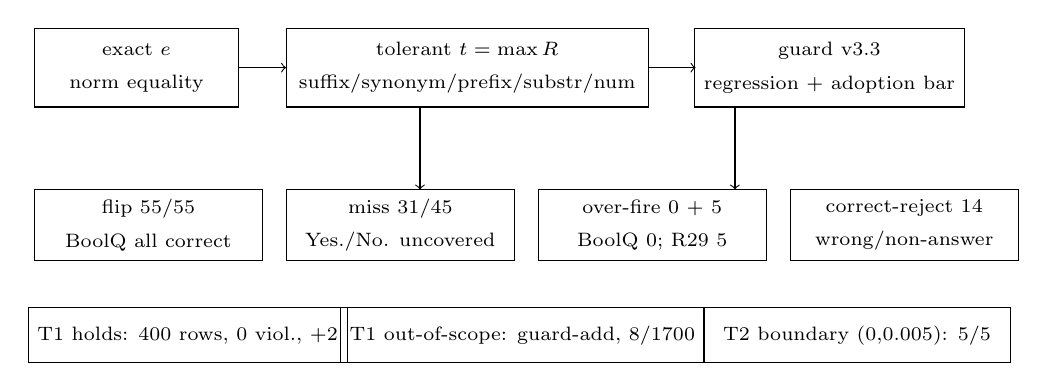
\begin{tikzpicture}[x=1cm,y=1cm]
\node[draw,rectangle,minimum width=2.6cm,minimum height=1.0cm,align=center] (e) at (1.4,3.4) {\scriptsize exact $e$\\\scriptsize norm equality};
\node[draw,rectangle,minimum width=4.6cm,minimum height=1.0cm,align=center] (t) at (5.6,3.4) {\scriptsize tolerant $t=\max R$\\\scriptsize suffix/synonym/prefix/substr/num};
\node[draw,rectangle,minimum width=3.4cm,minimum height=1.0cm,align=center] (g) at (10.2,3.4) {\scriptsize guard v3.3\\\scriptsize regression + adoption bar};
\draw[->] (2.7,3.4) -- (3.3,3.4);
\draw[->] (7.9,3.4) -- (8.5,3.4);
\node[draw,rectangle,minimum width=2.9cm,minimum height=0.9cm,align=center] (f) at (1.55,1.4) {\scriptsize flip 55/55\\\scriptsize BoolQ all correct};
\node[draw,rectangle,minimum width=2.9cm,minimum height=0.9cm,align=center] (m) at (4.75,1.4) {\scriptsize miss 31/45\\\scriptsize Yes./No. uncovered};
\node[draw,rectangle,minimum width=2.9cm,minimum height=0.9cm,align=center] (o) at (7.95,1.4) {\scriptsize over-fire 0 + 5\\\scriptsize BoolQ 0; R29 5};
\node[draw,rectangle,minimum width=2.9cm,minimum height=0.9cm,align=center] (c) at (11.15,1.4) {\scriptsize correct-reject 14\\\scriptsize wrong/non-answer};
\draw[->] (5.0,2.9) -- (5.0,1.85);
\draw[->] (9.0,2.9) -- (9.0,1.85);
\node[draw,rectangle,minimum width=3.9cm,minimum height=0.7cm,align=center] (t1a) at (2.05,0.0) {\scriptsize T1 holds: 400 rows, 0 viol., +2};
\node[draw,rectangle,minimum width=4.1cm,minimum height=0.7cm,align=center] (t1b) at (6.3,0.0) {\scriptsize T1 out-of-scope: guard-add, 8/1700};
\node[draw,rectangle,minimum width=3.9cm,minimum height=0.7cm,align=center] (t2) at (10.55,0.0) {\scriptsize T2 boundary (0,0.005): 5/5};
\end{tikzpicture}
\caption{The measurement pipeline. Exact matching nests inside tolerant matching (disjunction over the rule set $R$); the v3.3 guard adds a regression plus adoption bars. Sealed row counts on the four exits: BoolQ arm 55 flips (all content-correct), 31 misses, 14 correct rejects, 0 over-fire (plus 5 R29 numeric over-fires); hetero arm 8 confirmed flips with 8/11 cross-family judge agreement; rule-addition monotonicity (T1) holds on 400 rows with 2 increments and excludes guard-adding revisions (8/1700 accept-to-reject); the numeric-tolerance boundary (T2) contains all 5 R29 over-fire rows.}
\label{fig:pipeline}
\end{figure}

\subsection{Outcomes and adjudication}

On identical rows we report accuracy, 10-bin ECE (ece10), flip count, and flip rate (flips divided by n). Formal definitions: for $B=10$ bins partitioning $[0,1]$, $\mathrm{ECE} = \sum_{b=1}^{B} (n_b/n)\,|\mathrm{acc}_b - \mathrm{conf}_b|$ with $n_b$ rows, empirical accuracy $\mathrm{acc}_b$, and mean confidence $\mathrm{conf}_b$ in bin $b$. Discordant pairs are reported as counts: $b$ exact-wrong/guarded-right and $c$ exact-right/guarded-wrong rows. No paired test is run: the guarded matcher nests the exact matcher (exact accept implies guarded accept on non-degenerate rows; cf.\ code, scripts/label\_match\_v33.py), so $c=0$ by construction and any McNemar p-value would be a definitional tautology ($p=2/2^b$). Layers with $b+c=0$ are reported as no discordants.

Binning disclosure: all ECE values in the main table use one equal-width 10-bin convention (bin $i$ is $(i/10,(i+1)/10]$ with $0$ in bin $0$, the Guo-style upper-edge-inclusive rule; scripts/recompute\_ece\_unified.py, results/ece\_unified.json; fourteen strata are housed there, and the hetero-family ECE pair (0.5143/0.381) is housed in results/r18\_heteromodel.json and results/r18\_heteromodel\_adjudication.json under the same ece\_equal\_width function). Earlier strata were sealed under two other conventions: equal-frequency bins on the prior strata (analysis\_d2.py) and a hand-rolled floor-bin equal-width variant on five live strata (scripts/analyze\_new60.py and its copies), whose sealed numbers are reproduced by a quirk-faithful replica (a \texttt{bins.index} aliasing quirk in the legacy function, documented in the recomputation script) and retained in the appendix for audit. The old ``0.1692 coincidence'' note is withdrawn: 0.1692 was the equal-frequency computation on guarded labels all along (results/guard\_v31.json and results/tempscale.json share function and labels), not a cross-convention coincidence; under the unified convention the cloud-new guarded ECE is 0.0558. The flip set (exact outcome differing from tolerant outcome) must be adjudicated row by row under a semantic-equivalence standard (does the prediction express the correct answer in gold, not string equality) before entering calibration analysis. The 16 prior flips were first adjudicated in-session and then re-adjudicated by a heterogeneous judge on the cloud host (qwen2.5:7b, temperature 0, evidence/cloud\_judge\_16.json): 16 of 16 judged correct for the tolerant matcher, in full agreement with the in-session ruling. The authoring model is muse-spark, so the judge is heterogeneous with respect to authorship. No external gold judge set exists; judge FNR/FPR are characterized on 220 sealed pairs plus 60 adversarial negatives (author-labeled formula-confusable and CJK-fragment items): all five judge configurations stay below the enable bar (results/judge\_calib\_report.json; local gemma3:4b posts FPR 0.9 on negatives and is disqualified as a correctness judge, local qwen2:7b posts FPR 0.35, deepseek-r1:7b posts FPR 0.05 but keeps a pilot false positive; no judge enabled; author grades carry measured reliability (Cohen $\kappa=0.91$ vs a blinded second rater on a 30-item subset, sole divergence H64 adjudicated against the author; results/rater2\_kappa.json)).

The 5 cloud-new flips were adjudicated by the same heterogeneous judge (evidence/cloud\_judge\_new60.json): 4 of 5 judged correct (numeric/unit/synonymy) and 1 judged incorrect (cloud-new-42, ``O'' vs ``O2'': atomic oxygen is not molecular oxygen, a substring over-match on a short chemical formula).

A confirmation re-run of all 21 prior flips on the cloud host with the identical prompt reproduced 16 of 16 and 4 of 5 with zero deviation (evidence/cloud\_judge\_confirm2.json); a shortened prompt variant once flipped pilot-30, and the original prompt re-tested 3 of 3 CORRECT, so the episode is prompt sensitivity rather than model instability. The 5 local-new flips were adjudicated in-session under the same standard (evidence/local\_adjudication.json): 5 of 5 correct (same-line confidence suffix, numeric tolerance, book-title brackets, unit suffix, full-name containment). The 4 local-big flips were adjudicated in-session under the same standard (evidence/big\_adjudication.json): 4 of 4 correct (trailing-decimal numeric equivalence). The English stratum triggered no adjudication (0 flips). A second-judge attempt for local-new with qwen3:4b failed on single-word instruction compliance (verdicts echoed the instructions and were discarded, never recorded as evidence); single-rater adjudication for the extension strata is disclosed as a limitation. A cloud test-retest of the same 60 cloud-new questions on the same model, prompt, and temperature (scripts/cloud\_retest60.py, evidence/cloud\_retest60\_raw.json, results/retest60.json) reaches exact-string agreement 0.9833 on 60 pairs and guarded agreement 1.0, with identical raw-basis flip sets (5 and 5, including the documented O2 mis-accept; guarded basis 4 and 4) and mean absolute confidence drift 0.0107; the single differing string preserves the flip state (exact-wrong and guarded-right in both runs), so the cloud-new adjudication carries over, and the paired McNemar comparison is degenerate (b=0, c=0, p=1.0, disclosed). A blinded gold set (GOLD-25: a census of all 14 flips carrying stems plus a seeded sample of 11 adjudication-core flips without archived stems, order shuffled, verdicts sealed in evidence/gold\_key.json) was graded blindly item by item by the author without access to guarded outcomes (gold\_grading\_pack.csv, grades\_gold25\_user.csv): the pre-registered decode reports 25 of 25 under its all-guarded-correct assumption (scripts/analyze\_gold.py, results/gold\_agreement.json), but that assumption fails on G06 (trace cloud-new-42, guarded-incorrect), so agreement against guarded outcomes is 24 of 25 (agreement 0.96, Wilson 95\% CI 0.805 to 0.993; 13 of 14 with stems, 11 of 11 stemless; scripts/recompute\_gold\_guarded.py, results/gold\_guarded\_agreement.json). Exact-match non-flip rows were excluded from the gold set by design (their answers equal the reference verbatim, hence zero information on overturn quality), and the set is flip-enriched rather than a random sample, so the 24 of 25 bounds overturn quality on flip strata only, with the single divergence disclosed above; GOLD-100 is stratified by design (not a random sample), contributes 9 guard false negatives outside the flip set (plus the H64 author slip) plus 1 sampled gold whose reference was factually wrong at sampling time and corrected post-hoc (H09), and its echo-exclusion divergences (H47/H85) cut against the sealed exclusion. A 100-item stratified extension (GOLD-100: all 7 exclusions plus 55 confirmed flips plus 38 non-flip rows including both-wrong negatives, blinded with the key sealed) was graded blindly by the author (gold100\_grading\_pack.csv, grades\_gold100\_user.csv, GOLD100\_README.md, evidence/gold100\_key.json, decode scripts/decode\_gold100.py; results/gold100\_agreement.json); see the GOLD-100 paragraph below for the decoded numbers. Adjudication accounting convention (used identically in the Abstract, Contributions, and every stratum paragraph): judged counts every row submitted to any judge pass, including 4 non-flip probe rows carried as controls (R18 lr18-42 plus hetero-family gr18-41/42/45, all judge-rejected and guard-rejected under v3.3); confirmed counts rows accepted correct on content in the final ruling. Canonical rollup: 106 judged (102 flip rows plus 4 probes), 99 confirmed (scripts/seal\_R25\_numbers.py, results/adjudication\_recount\_R25.json).

A component ablation (scripts/ablation.py, results/ablation.json) attributes each of the 16 prior flips to the earliest-firing v3 rule: synonymy 7, numeric tolerance 4, unit suffix 3, substring 1, negation prefix 1.

A two-rule substring guard (v3.3, scripts/label\_match\_v33.py, results/guard\_v33.json; v3.1 formula rule plus the R22 single-CJK-character rule) refuses substring acceptance exactly when both normed sides match \texttt{\^{}[a-z0-9]\{1,4\}\$} while differing with minimum length at most 2 (short-ASCII formula-confusable pairs such as ``O'' vs ``O2''); such pairs fall through to numeric equivalence, which rejects them. Multi-character CJK name pairs are non-ASCII and unaffected by either rule; single-character CJK sides are blocked by the v3.3 rule and fall through to numeric equivalence, which rejects them. Circularity disclosure: the guard was constructed after seeing the 120-row adjudication, so its exact reproduction of those labels is in-sample by construction; its out-of-sample support comes from the fresh-question power-replication arms (10 of 10 flips confirmed correct, zero guard-triggered disputes) and the 470-row zero-difference regression, not from the fit itself; a synthetic targeting test now measures the boundary (see evidence pointers): formula recall and precision 12 of 12, accept specificity 12 of 12, CJK-fragment catch 8 of 8 under the v3.3 patch (8 of 8 missed before it).

A v3.2 revision (scripts/label\_match\_v32.py, results/guard\_v32.json) adds a single raw-fallback inside the empty-answer guard: when both raw answers are non-empty but both normalize to empty, the decision falls back to stripped-raw equality. The 470-row regression against v3.1 shows zero decision differences with zero unexpected outcomes, so v3.1 remains the reported basis and v3.2 is the current vendored implementation with identical decisions on all existing evidence.

A temperature-scaling comparison (scripts/tempscale.py, results/tempscale.json) fits a scalar temperature per stratum on adjudicated labels (confidence clipping 1e-6, temperature bounds 0.05 to 20) and reports NLL plus equal-frequency 10-bin ECE at temperature 1 versus the fitted temperature.

\subsection{Descriptive analysis plan and sensitivity context}

All paired reporting is descriptive: flip counts, flip rates, and $b$/$c$ cells, with no significance test run for the nesting reason above. Power ceilings computed under the placeholder odds ratio of 4 (disclosed as a placeholder, unchanged from pre-registration; analysis\_plan\_power\_rep.md) are retained as sensitivity context only, not as pre-data justifications: pilot n\_ceil=50 (current 30; unmet, no top-up available, reported as descriptive pilot data only), holdout-main n\_ceil=108 (current 30), cloud-new n\_ceil=217 (current 60), local-new n\_ceil=217 (current 60), local-big n\_ceil=720 (current 160), local-en not powered (0 discordants). The same-model pool (local-new plus local-big, n=220) is a pre-specified composition reported descriptively (9 flips of 220, rate 0.0409). A Holm-Bonferroni accounting over the eighteen paired comparisons is sealed (results/holm.json) and reported for completeness; under the nested construction it carries no inferential license (see the Holm accounting appendix). The recomputation scripts are paper\_workflow\_kb/analysis\_d2.py (prior 60), scripts/analyze\_new60.py (cloud-new), scripts/analyze\_local60.py (local-new), and scripts/analyze\_big\_en.py (local-en, local-big, and the pool).

\subsection{External validation (R26, descriptive)}

A pre-registered external validation (PREREG\_R26\_EXTERNAL.md, frozen before any download or answering) checks whether the guard's miss behavior transfers outside the curated answer-style pool. Two public short-answer sets are sampled with a frozen shuffle seed (20260908): TriviaQA-RC (wikipedia dev) and EntityQuestions (test), 200 questions each with gold alias sets (scripts/r26\_sample.py; evidence/r26\_trivia\_sample.jsonl, evidence/r26\_entity\_sample.jsonl, SHA-256 in the manifest). A local model (qwen2:7b, temperature 0, the same pooled local-family model) answers each question (results/r26\_answers\_trivia.jsonl, results/r26\_answers\_entity.jsonl); every prediction is scored by exact match and by guard v3.3 against the alias set, and a candidate v3.4 (v3.3 plus a token-containment fallback: every token of any gold alias appears in the prediction, or vice versa) is scored on the same rows. Flip rows (exact-reject, guard-accept) are adjudicated row by row by the author (the over-fire count); a seeded sample of 60 guard-rejected rows per set is adjudicated against the aliases to estimate the miss rate (Wilson 95\% CI, descriptive). Distribution difference is disclosed up front: these are public factual-question sets, not the numeric/unit/synonym/name-variant answer styles on which the guard was built, so the external counts describe the guard's transfer, not a recalibration of the main accuracy or ECE cells, and no calibration claim attaches to these sets. Descriptive outcome (results/r26\_seal.json, unique recomputation scripts/seal\_R26.py): on the 200 trivia rows exact/guard are 95/123, 3 over-fire in 28 flips, and a 2-of-60 miss rate (Wilson 95\% CI 0.0092--0.1136); on the 200 entity rows 25/57, 2 over-fire in 32 flips, and a 0-of-60 miss rate (CI 0.0--0.0602). The candidate v3.4 drops the combined miss by 2 (entity 0, trivia 2) with zero over-fire increase, short of the frozen adoption bar (miss drop \(\geq5\) and over-fire increase \(\leq2\)), so v3.4 is not cut and v3.3 remains the guarded baseline (a pre-registered negative result).

\section{Results}
\label{sec:results}

\subsection{Stratified outcomes}

Table~\ref{tab:stratified} gives the stratified recomputed values from results/analysis.json (prior strata), results/cloud\_new.json (cloud-new), results/local\_new.json (local-new), results/local\_en.json (local-en), results/local\_big.json (local-big), results/xdomain.json (cross-domain tight and loose), results/powrep.json (power-replication arms), results/powrep\_rollups.json (extended strata), results/combined\_qwen2.json (pre-specified pool), results/r18\_heteromodel.json (hetero-family raw), results/r18\_heteromodel\_adjudication.json (hetero-family adjudicated), and results/merged\_1062.json (descriptive merged sums). Figure~\ref{fig:acc} visualizes the exact-versus-guarded accuracy gap per stratum. The fourteen result files present at that check were re-executed on the cloud host with byte-identical outputs (scripts/cloud\_repro\_check.py, results/cloud\_repro.json); strata added later (cross-domain, power-replication, Holm, gold-guarded, R18, hetero-family, unified-binning) are verified by their own sealed scripts, not by that check. Methods and Results use these values only; the Discussion follows; the Abstract was written last to match them.

\begin{table}[t]
\caption{Stratified outcomes on the guarded basis (v3.3 guarded basis throughout; v3.1 strata 1--12 and v3.2 strata 13--15 identical on their rows; N=1062 in fifteen strata; reporting is stratified and descriptive only, no tests run; raw-tier cloud-new: 5 flips, ECE 0.0425, see text; R18 adjudicated: 24 flips (raw 26), see text; hetero adjudicated: 8 flips (raw 8), hetero ECE exact-column raw-basis and guarded-column adjudicated-basis, see text; loose-regime reruns reported in text, excluded from N; ECE uses rows carrying confidences only: local-new 55 of 60, local-big 156 of 160; all ECE are equal-width 10-bin under one convention (upper-edge inclusive); fourteen strata housed in results/ece\_unified.json (scripts/recompute\_ece\_unified.py), hetero pair in results/r18\_heteromodel.json and results/r18\_heteromodel\_adjudication.json under the same function; equal-frequency values are retained in the appendix for audit)}
\label{tab:stratified}
\begin{center}
{\footnotesize\setlength{\tabcolsep}{3pt}
\begin{tabular}{lcccccc}
\hline
Subset & n & Acc exact & Acc guarded & ECE exact & ECE guarded & Flips (rate; b/c) \\
\hline
Pilot & 30 & 0.6333 & 1.0 & 0.363 & 0.0037 & 11 (0.3667; b=11, c=0) \\
Holdout-main & 30 & 0.6333 & 0.8 & 0.3317 & 0.165 & 5 (0.1667; b=5, c=0) \\
Cloud-new & 60 & 0.8 & 0.8667 & 0.1075 & 0.0558 & 4 (0.0667; b=4, c=0) \\
Local-new & 60 & 0.8 & 0.8833 & 0.1255 & 0.0782 & 5 (0.0833; b=5, c=0) \\
Local-en & 30 & 1.0 & 1.0 & 0.08 & 0.08 & 0 (0.0; b=0, c=0) \\
Local-big & 160 & 0.925 & 0.95 & 0.0413 & 0.0542 & 4 (0.025; b=4, c=0) \\
Math & 40 & 0.925 & 0.925 & 0.025 & 0.025 & 0 (0.0; b=0, c=0, no discordants) \\
XDomain-tight & 60 & 0.8333 & 0.85 & 0.0533 & 0.0367 & 1 (0.0167; b=1, c=0) \\
XDomain-loose & 60 & 0.4167 & 0.75 & 0.4767 & 0.1433 & 20 (0.3333; b=20, c=0) \\
PowPilot & 20 & 0.8 & 0.8 & 0.13 & 0.13 & 0 (0.0; b=0, c=0, no discordants) \\
PowHoldout & 78 & 0.9103 & 0.9359 & 0.0261 & 0.0517 & 2 (0.0256; b=2, c=0) \\
PowCloudNew & 157 & 0.9108 & 0.9172 & 0.0204 & 0.0268 & 1 (0.0064; b=1, c=0) \\
PowLocalNew & 157 & 0.8917 & 0.9363 & 0.0349 & 0.0668 & 7 (0.0446; b=7, c=0, single-arm, no power conclusion) \\
R18-loose-rep & 60 & 0.25 & 0.65 & 0.6425 & 0.2425 & 24 (0.40; b=24, c=0, adjudicated; raw 26) \\
Hetero-gemma & 60 & 0.35 & 0.4833 & 0.5143 & 0.381 & 8 (0.1333; b=8, c=0, adjudicated; raw 8) \\
\hline
\end{tabular}
}
\end{center}
\end{table}

\begin{figure}[t]
\centering
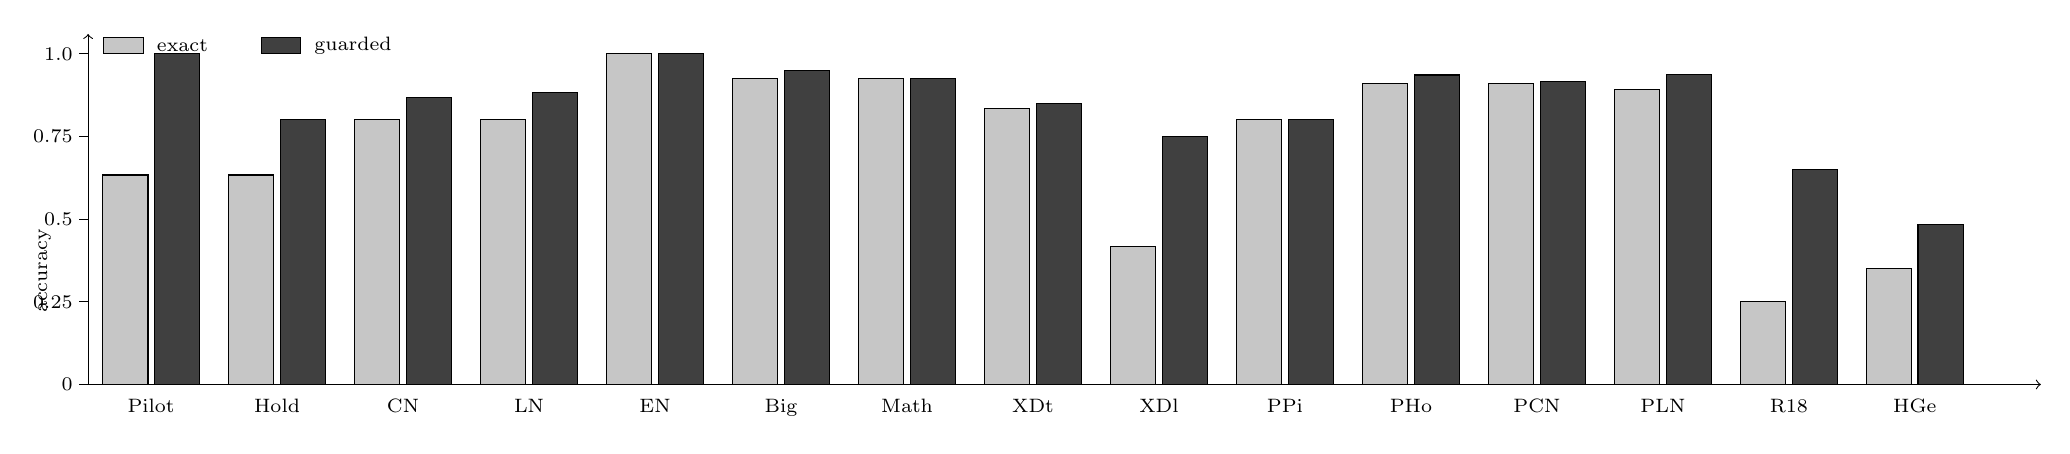
\begin{tikzpicture}[x=1cm,y=4.2cm]
\draw[->] (0,0) -- (24.8,0);
\draw[->] (0,0) -- (0,1.06);
\foreach \y in {0,0.25,0.5,0.75,1.0} {\draw (0,\y) -- (-0.12,\y) node[left,inner sep=2pt] {\scriptsize \y};}
\node[left,rotate=90] at (-0.55,0.5) {\scriptsize accuracy};
\newcommand{\pairbar}[4]{\draw[fill=gray!45] (#1-0.62,0) rectangle (#1-0.04,#3); \draw[fill=black!75] (#1+0.04,0) rectangle (#1+0.62,#4); \node[below] at (#1,-0.015) {\scriptsize #2};}
\pairbar{0.8}{Pilot}{0.6333}{1.0}
\pairbar{2.4}{Hold}{0.6333}{0.8}
\pairbar{4.0}{CN}{0.8}{0.8667}
\pairbar{5.6}{LN}{0.8}{0.8833}
\pairbar{7.2}{EN}{1.0}{1.0}
\pairbar{8.8}{Big}{0.925}{0.95}
\pairbar{10.4}{Math}{0.925}{0.925}
\pairbar{12.0}{XDt}{0.8333}{0.85}
\pairbar{13.6}{XDl}{0.4167}{0.75}
\pairbar{15.2}{PPi}{0.8}{0.8}
\pairbar{16.8}{PHo}{0.9103}{0.9359}
\pairbar{18.4}{PCN}{0.9108}{0.9172}
\pairbar{20.0}{PLN}{0.8917}{0.9363}
\pairbar{21.6}{R18}{0.25}{0.65}
\pairbar{23.2}{HGe}{0.35}{0.4833}
\draw[fill=gray!45] (0.2,1.0) rectangle (0.7,1.05); \node[right] at (0.75,1.025) {\scriptsize exact};
\draw[fill=black!75] (2.2,1.0) rectangle (2.7,1.05); \node[right] at (2.75,1.025) {\scriptsize guarded};
\end{tikzpicture}
\caption{Exact versus guarded accuracy across all fifteen strata (N=1062). The gap is the flip mass: largest on the pilot (0.6333 to 1.0), the loose cross-domain layer (0.4167 to 0.75), the R18 loose replication (0.25 to 0.65 adjudicated), and the hetero-family replication (0.35 to 0.4833 adjudicated); zero on the English, math, and pilot-replication arms. ECE moves per stratum are in Table~\ref{tab:stratified}.}
\label{fig:acc}
\end{figure}

Pilot: 19 of 30 exact-correct versus 30 of 30 tolerant-correct (identical to guarded on this stratum); 11 flips, flip rate 0.3667, b=11, c=0 (descriptive; no test run). The flip rate clears the descriptive bar (0.3667 exceeds 0.05); D1 is reported descriptively (pilot n=30 of pre-specified 50; top-up to 50 pending). ECE moves from 0.363 to 0.0037 conditional on the adjudicated flip set. The heterogeneous judge confirmed all 11 flips correct for the tolerant matcher.

Holdout-main: 19 of 30 exact-correct versus 24 of 30 tolerant-correct (identical to guarded on this stratum); 5 flips, flip rate 0.1667, b=5, c=0 (descriptive). The descriptive bar is cleared; with no inferential test run, the conclusion stays hedged. ECE moves from 0.3317 to 0.165 conditional on the adjudicated flip set. The heterogeneous judge confirmed all 5 flips correct for the tolerant matcher (holdout-7 numeric tolerance 8848.86m vs 8848; holdout-10 numeric tolerance 365.25 vs 365; holdout-23/25/26 synonymy ``不会''/``不是'' vs ``否'').

Cloud-new: 48 of 60 exact-correct versus 53 of 60 tolerant-correct (raw); 5 flips, flip rate 0.0833 raw, b=5, c=0 (descriptive). D1 clears the descriptive bar only (0.0833 exceeds 0.05). ECE moves from 0.1075 to 0.0425 on raw matcher output. The heterogeneous judge confirmed 4 of 5 flips correct and 1 incorrect (cloud-new-42 ``O'' vs ``O2''); adjudicated tolerant accuracy is therefore 52 of 60 for this stratum.

Local-new: 48 of 60 exact-correct versus 53 of 60 guarded-correct; 5 flips, flip rate 0.0833, b=5, c=0 (descriptive). D1 clears the descriptive bar only (0.0833 exceeds 0.05), replicating the cloud-new pattern on the same questions with a different model. ECE moves from 0.1255 to 0.0782 on the 55 rows carrying confidences. In-session adjudication confirmed all 5 flips correct (same-line confidence suffix, numeric tolerance, book-title brackets, unit suffix, full-name containment); the failed qwen3:4b second-judge attempt is disclosed in Methods and this stratum stays single-rater.

Guarded rerun (v3.1): across the first 120 rows the guard changes exactly one decision (cloud-new-42 now rejected) with zero regressions (pilot-03 and cloud-new-48 name pairs still accepted). Guarded cloud-new accuracy is 52 of 60 (0.8667), identical as a set to the adjudicated labels; guarded flips are 4 of 60 (0.0667, b=4, c=0, descriptive). Guarded cloud-new ECE is 0.0558: the raw 0.0425 was flattered by the false accept, and the adjudicated ECE is reported as-is. Pilot and holdout-main are unchanged by the guard (11 and 5 flips, same b/c counts). Local-new was analyzed directly on the guarded basis (5 flips, all confirmed correct); no guarded-vs-v3 difference was asserted there because v3 was never the reported basis for this stratum. A synthetic boundary probe (see evidence pointers for script and results; author-labeled ground truth, disclosed) measures the guard where real data cannot: formula-confusable recall 12 of 12 blocked with precision 12 of 12 (zero over-fire on 12 true accepts spanning norm-equality, suffix, synonym, and same-person CJK containment), and CJK single-character fragments missed 8 of 8 by construction under v3.1/v3.2 (non-ASCII never matches the short-ASCII rule; 4 observed plus 4 author-labeled subtypes). The v3.3 patch (R22: block substring acceptance for single-CJK-character sides, appendix) catches all 8 synthetic fragments with zero over-fire (accept specificity stays 12 of 12, formula recall/precision 12 of 12). On real data the guard accepts all 92 confirmed flips and all 3 in-sample regression anchors, catches the G06 formula false positive and the 4 single-character exclusions (lr18-42, gr18-41/42/45), and misses only the 2 echo-containment exclusions (lr18-54/55, judge-majority against the author-noted correct ruling); v3.2 and v3.3 differ on exactly the 11 probed single-CJK rows (8 synthetic plus 3 hetero-excluded) of 130.

Temperature scaling on adjudicated labels: fitted temperatures are 0.207 (pilot), 6.3983 (holdout-main), and 1.7756 (cloud-new). NLL improves in all strata, but ECE under the unified equal-width convention does not improve consistently: 0.0037 to zero (pilot, degenerate all-correct stratum), 0.165 to 0.1147 (holdout-main, improves), 0.0558 to 0.1384 (cloud-new, worsens). The NLL-optimal temperature is not consistently ECE-optimal on these rows; temperature scaling is a partial fix at best, and this mixed result is reported without a repair claim. (Equal-frequency values for audit: 0.205 to 0.2805 on holdout-main, 0.1692 to 0.2272 on cloud-new; see appendix.)

Isotonic regression on the same adjudicated labels (hand-rolled count-weighted PAV on confidence-sorted rows, scripts/isotonic.py, results/isotonic.json; equal-width recomputation in results/ece\_unified.json) collapses in-sample ECE to zero on all three strata (fitted block means are bin-constant, so the in-sample column is uninformative by construction) and fails under honest 5-fold cross-validation (holdout-main CV ECE 0.1934 against raw 0.165; cloud-new CV ECE 0.1172 against raw 0.0558 with CV NLL worsening 35.2309 to 61.9291, small-sample overfit; pilot stays degenerate at zero). In-sample optimism is disclosed; the CV column governs. Jointly, the two standard post-hoc fixes offer no consistent ECE repair on near-degenerate confidences (temperature scaling helps one stratum and hurts another; isotonic regression fails held-out ECE on both informative strata); the label-side guard is the repair that worked. Disposition at n=157 (scripts/dispose\_n157.py, results/tempiso\_n157.json; same NLL fits and PAV-CV machinery on the two 157-row power-replication arms under v3.2-guarded labels, unified equal-width): PowCloudNew temperature barely moves (T*=0.8928, ECE 0.0268 to 0.0241) and isotonic CV worsens (0.0351 with CV NLL 46.111 to 76.8072, overfit again); PowLocalNew temperature improves NLL (73.5696 to 69.566) but worsens ECE (0.0668 to 0.1407), while isotonic CV improves both ECE (0.0668 to 0.0277) and NLL (to 57.1359) — the single non-trivial positive among the five isotonic held-out (5-fold CV) ECE tests (pilot, holdout-main, cloud-new, PowCloudNew, PowLocalNew; pilot moves 0.0037 to 0.0 in a degenerate all-correct stratum and is uninformative), reported plainly. Larger n does not rescue consistency.

Local-en: 30 of 30 exact-correct; 0 flips, flip rate 0.0, b=0, c=0. Neither the descriptive bar nor D1 is met here: on clean English short answers the exact matcher already decides everything, so this stratum is a reported boundary condition and triggers no adjudication. ECE is 0.08 on either basis.

Local-big: 148 of 160 exact-correct versus 152 of 160 guarded-correct; 4 flips, flip rate 0.025, b=4, c=0 (descriptive). The descriptive bar is missed (0.025 below 0.05) on this arithmetic-heavy stratum. ECE moves from 0.0413 to 0.0542 on the 156 rows carrying confidences. In-session adjudication confirmed all 4 flips correct (trailing-decimal numeric equivalence).

Pre-specified pool: local-new plus local-big share model, temperature, and matcher basis (n=220; post-hoc n\_ceil=217, composition pre-specified). The pool flips 9 of 220 (0.0409, b=9, c=0, descriptive; no test run). The descriptive bar (>5\%) is missed while the b-cell count stands as observed; only the pool composition was pre-specified.

Math (cloud, second question family): 37 of 40 exact-correct versus 37 of 40 guarded-correct; 0 flips, no discordants (b=0, c=0). Neither the descriptive bar nor D1 is met on pure numeric questions: with no units, synonyms, or names in play, exact and guarded matchers agree everywhere. ECE is 0.025 on both bases. No adjudication is required (zero flips fall below the adjudication gate's 5\% bar); a power ceiling is not computable from zero discordant pairs and none is plugged in.

Cross-domain tight (cloud, same 60 questions, format-constrained prompt): 50 of 60 exact-correct versus 51 of 60 guarded-correct; 1 flip, flip rate 0.0167, b=1, c=0 (descriptive). The descriptive bar is missed (0.0167 below 0.05) under tight instructions, replicating the local-big pattern on a new domain. ECE moves from 0.0533 to 0.0367. The single flip (``东坡居士'' vs ``东坡'', full-title containment) was confirmed correct by the heterogeneous judge.

Cross-domain loose (cloud, same 60 questions, paraphrase-regime prompt): 25 of 60 exact-correct versus 45 of 60 guarded-correct; 20 flips, flip rate 0.3333, b=20, c=0 (descriptive; no test run). The flip rate clears the descriptive bar: loosening the instruction format recovers the paraphrase surface (unit suffixes, yes-no synonymy with same-line confidence particles, name containment) that tight instructions suppress. ECE moves from 0.4767 to 0.1433. This is the largest observed flip count in the paper; the layer is post-registration (the loose direction was a documented intent in the collection script docstring before running it, not a sealed pre-registration) with no pre-specified n\_ceil, reported with the same pilot-class observed status as the pilot. A v3.2 versus v3.3 decision check on all 120 cross-domain rows shows zero differences, so the table reports the v3.3 basis. Overlap disclosure: 5 of the 60 questions share core stems with pre-existing rows under different format hints (results/xdomain\_sensitivity.json); excluding them leaves tight at 1 of 55 (b=1, c=0) and loose at 19 of 55 (b=19, c=0), so the main conclusion does not depend on those 5 rows.

Cross-domain adjudication (heterogeneous judge family: local deepseek-r1:7b versus the cloud qwen2.5:7b collection model, temperature 0; evidence/xdomain\_judge.json, evidence/xdomain\_judge\_pass2.json, sealed counts results/xdomain\_adjudication.json): first pass 16 correct, 3 incorrect, 2 timeouts on 21 flips; all 3 incorrects carry a same-line confidence leak (``不是。0.9'' vs ``否'', ``是的。0.9'' vs ``是'') while leak-free siblings pass, identifying a protocol artifact rather than a semantic failure. A second pass strips the trailing confidence float and re-judges exactly those 5 rows: 5 of 5 correct. Content-basis adjudication is therefore 21 of 21; both passes stay on record.

Power-replication arms (fresh de-duplicated questions, v3.3 basis identical to v3.2 on these rows): PowPilot 16 of 20 exact-correct versus 16 of 20 guarded-correct (0 flips, degenerate); PowHoldout 71 of 78 versus 73 of 78 (2 flips, 0.0256, b=2, c=0); PowCloudNew 143 of 157 versus 144 of 157 (1 flip, 0.0064, b=1, c=0); PowLocalNew 140 of 157 versus 147 of 157 (7 flips, 0.0446, b=7, c=0, single-arm observation; one of four observed arms with few discordant pairs, so no power conclusion is drawn). ECE moves are small on all four arms (all under 0.07 on either basis). The heterogeneous judge (local deepseek-r1:7b) confirmed all 10 flips correct, including one numeric-tolerance accept well within the 0.5\% relative-error tolerance (999 vs 1000, same standard as the pilot precedent) and one re-judgment after a strip-rule bug fix (a 40.0 answer mangled to 4 by the first strip rule; fixed rule requires separator-adjacency, true form re-judged correct, both records kept).

R18 loose-rep (cloud, pre-registered, 60 fresh questions, v3.3 basis): 15 of 60 exact-correct versus 41 of 60 guarded-correct (raw); 26 flips, flip rate 0.4333, b=26, c=0 (descriptive, no test run). The directional expectation (loose flip rate above comparable tight layers on paraphrase-surface questions) is confirmed descriptively: 26 of 60 exceeds the xdomain-loose 20 of 60 on the same prompt verbatim. ECE moves from 0.6425 to 0.2092 raw. Adjudication by the heterogeneous judge (local deepseek-r1:7b, temperature 0; evidence/r18\_judge.json, pass2, pass2b, pass2c; rollup results/r18\_adjudication.json): pass 1 confirms 17 of 27 rows put to the judge (26 raw flips plus the lr18-42 non-flip control); a leak-stripped second pass confirms 5 more (xdomain precedent); a retry pass moves lr18-54 to correct but the clean-read majority (1c/2i) still excludes it; a bilingual-parser pass confirms 1 (lr18-34, the judge had answered in Chinese); lr18-46 stays judge-ERROR across four attempts and is author-ruled correct under the echo standard (cf.\ confirmed lr18-47/51), disclosed. Final: 24 of 26 confirmed on content; excluded are lr18-54 and lr18-55 (judge-rejected echo-containment despite full gold containment, an instrument inconsistency against the accepted lr18-47/51 echoes; author-correct rulings noted). The former second false-positive exemplar lr18-42 (``牧'' vs ``牧之'') is now rejected by the v3.3 guard itself (its judge-rejection call retained on record; non-flip under v3.3). Adjudicated guarded accuracy is 39 of 60 (0.65), adjudicated flips 24 of 60 (0.40), adjudicated ECE 0.2425 equal-width. Hetero-family replication (local gemma3:4b, same xdomain 60 questions, verbatim loose prompt, mini-pre-registered): 21 of 60 exact-correct versus 29 of 60 guarded-correct (raw); 8 flips, flip rate 0.1333, b=8, c=0 (descriptive, no test run). The directional expectation (flips above zero on paraphrase-surface questions in a different model family) is confirmed descriptively. Adjudication by the heterogeneous judge (local qwen2.5:7b, temperature 0; evidence/r18\_heteromodel\_judge.json; rollup results/r18\_heteromodel\_adjudication.json): 8 of 8 flips confirmed on content (11 rows put to the judge); gr18-41, gr18-42, and gr18-45 (single-character fragments) are judge-rejected and now also guard-rejected under v3.3 (non-flips; the former third and fourth exemplars are closed by the patch). A second independent judge family (local deepseek-r1:7b, temperature 0, verbatim prompt, think allowed as disclosed, pre-registered in PREREG\_R31\_HETEROJUDGE.md; evidence/r18\_heteromodel\_judge2.json) re-judges the same 11 rows: 8 of 11 agree with the first judge (disagreements gr18-42/56, one ERROR gr18-09 after three attempts) and 8 of 11 agree with the sealed conclusion; disagreement on excluded rows is 1 of 3, below the pre-registered Limitations bar, so the sealed adjudication stands and the hetero stratum now carries cross-family reliability evidence rather than a single-rater verdict (results/r18\_heteromodel\_judge2\_agreement.json, scripts/seal\_heteromodel\_judge2.py). Adjudicated guarded accuracy is 29 of 60 (0.4833), adjudicated flips 8 of 60 (0.1333), adjudicated ECE 0.381 equal-width. This stratum is descriptive-only and excluded from the Holm family (no new comparison is added).

Extended strata (prior sealed stratum plus power-rep arm, deterministic rollup results/powrep\_rollups.json): pilot 11 of 50 flips (b=11, c=0; cross-model pool of pilot 30 plus PowPilot 20, descriptive only with no p-value claimed; the pilot D1 rests on the 30-row stratum); holdout 7 of 108 (b=7, c=0, single-arm observation with observed status and no power conclusion); cloud-new 5 of 217 guarded (b=5, c=0; raw basis 6 of 217); local-new 12 of 217 (b=12, c=0, observed status). These are two further observed readings in the paper; both carry pilot-class observed status because the extension rows are post-registration, and because the rollup rows overlap strata already tested, rollups are descriptive re-views outside the Holm family rather than new tests (cf. Multiplicity accounting).

Loose-regime rerun (same 255 power-rep questions, paraphrase-regime prompt, excluded from N like the retest): Pow1L 88 of 98 versus 90 of 98 (2 flips, b=2, c=0); Pow2L 145 of 157 versus 146 of 157 (1 flip, b=1, c=0); PowLL 143 of 157 versus 147 of 157 (4 flips, b=4, c=0); 7 of 7 confirmed correct in one clean pass. Against the tight arms on identical questions (3 and 7 flips), the prompt-regime contrast seen on the cross-domain set (1 versus 20) does not replicate: flip-rate heterogeneity is question-type-dependent, not a universal instruction switch. Collection had zero errors on both regimes (412 of 412 tight, 412 of 412 loose); the analyzed loose arms sum to the full 412 rows.

Test-retest stability (cloud, same 60 questions): exact-string agreement 0.9833 on 60 pairs, guarded agreement 1.0, identical raw-basis flip sets (5 and 5, including the documented O2 mis-accept; guarded basis 4 and 4), mean absolute confidence drift 0.0107, no discordants (b=0, c=0). The flip phenomenon is not single-sample jitter: the same five questions flip in both runs.

Blinded gold grading (GOLD-25): blinded item-by-item grading agrees 24 of 25 with guarded outcomes (agreement 0.96, Wilson 95\% CI 0.805 to 0.993; 13 of 14 with stems, 11 of 11 stemless; results/gold\_guarded\_agreement.json). The pre-registered decode assumed all 25 guarded-correct; that assumption fails on exactly one item, G06 (trace cloud-new-42, ``O'' vs ``O2''), which the pack builder drew from the raw flip file while the guarded verdict rejects it: the blinded grader accepted the response while guarded says incorrect. The remaining 24 cover flips from five flip-carrying strata known at grading time (the cross-domain layers came later). The extension flip rows are included in the 14 stem items, giving them a blinded second grading beyond the in-session single rater. Blinding note: the single blinded grader is the author, grading item-by-item without access to guarded outcomes; the 11 of 11 stemless grades are therefore author grades with no external check, reported as-is.

Blinded gold grading (GOLD-100): a 100-item stratified extension (census of all 7 excluded flips, 55 confirmed flips, 38 non-flip rows including both-wrong negatives; blinded order, key sealed in evidence/gold100\_key.json) was graded blindly item by item by the author without access to guarded outcomes (gold100\_grading\_pack.csv, grades\_gold100\_user.csv; scripts/decode\_gold100.py, results/gold100\_agreement.json; second-rater overlap grades\_rater2\_user2.csv with results/rater2\_kappa.json ($\kappa=0.91$ on 30 items; the second rater is an external human volunteer, not an author)). Agreement against guarded outcomes is 90 of 100 (0.9, Wilson 95\% CI 0.8256 to 0.9448; 71 of 79 with stems; flips 62 of 62, CI 0.9417 to 1.0). All 55 confirmed flips are accepted, and all 7 excluded rows now agree on the exact basis (H34, agreed as both-wrong by both blinded raters, triple-consistent with the guard's formula rejection; H47/H85, siding with the guard against the sealed exclusion; H62/H68/H71/H82, single-character CJK fragments the v3.3 guard itself rejects, matching the blind grader), so agreement against sealed adjudicated outcomes is 88 of 100 (95\% CI 0.8019 to 0.93), diverging only on the two echo-containment exclusions (H47/H85, lr18-54/55) where the blind grader sides with the guard --- and with the author's noted correct-ruling --- against the sealed exclusion. The remaining 9 divergences are guard false negatives on non-flip rows the grader accepts (unit and 朝-suffix variants, Jakarta/雅加达 transliteration, echo-plus-confidence-leak rows): a new limitation, since the flip-centric design does not surface matcher misses outside the flip set. A tenth apparent divergence (H64, ``支持'' vs ``是'') is an author grading slip, not a matcher miss: the blinded second rater rejects it with the guard (S09 grades 错), so the human gold is adjudicated 错 (2:1 with guard consistency); decode and P2-calibration numbers are unchanged (the decode keys off the recorded author grade vs guarded outcomes, and P2 covers flip rows only, H64 being a nonflip). One sampled gold reference was factually wrong at sampling time (H09 reference 是; ginger is a rhizome, not a root --- a blinded second rater independently flagged the same botanical dispute while still grading the response-vs-gold cell 错 under the stated gold) and is corrected post-hoc to 否 in R20 (gold100\_grading\_pack.csv); the agreement cell follows the sealed guarded outcome (错), which now disagrees with the corrected reference, so the row is retained as a seal artifact for audit. No number moves: the decode keys off guarded outcomes, not reference text (scripts/decode\_gold100.py). The set is stratified by design, not a random sample, so these rates bound grading agreement on the sampled rows only.

Merged 1062-pair numbers are descriptive only (830 exact-correct, 922 guarded-correct on the adjudicated basis, 92 flips, flip rate 0.0866). No merged inference of any kind is claimed. Coincidences are reported without merged inference: pilot and holdout-main show 19 of 30 exact-correct; cloud-new and local-new show 48 of 60 exact-correct.

\subsection{Cross-domain extension (R28)}

A pre-registered cross-domain extension (PREREG\_R28\_CROSSDOMAIN.md) tests the boundary predictions of the measurement-error formalization on two non-Chinese short-answer arms. Arm ``degenerate'' (40 local arithmetic items, pure-numeric gold) posts 1 of 40 flips: the sole flip ``125.0'' vs ``125'' is a numeric ``.0'' suffix accepted by the numeric-equivalence branch, so pure-numeric answers flip only through numeric-format alternates---near-zero, as prediction (i) predicts. Arm ``uncovered'' (40 English unit/count items, pure-numeric gold) posts 0 flips but 21 of 40 misses (Wilson 95\% CI 0.375--0.6706): the model emits English-unit variants (``60 seconds'', ``52 weeks'', ``2000 pounds'') that exact rejects and, because the unit-suffix and synonym lists are Chinese-specific, tolerant also rejects, so uncovered variants yield misses, not flips, confirming prediction (ii) (results/r28\_seal.json, scripts/r28\_seal.py, scripts/r28\_collect.py, scripts/r28\_adjudicate.py).

\subsection{Public yes/no arm (R30, BoolQ)}

A pre-registered public-dataset arm (PREREG\_R30\_BOOLQ.md) tests predictions (ii) and (iii) inside a single dataset: 100 BoolQ dev questions (SuperGLUE official package, stratified 50 True plus 50 False, frozen seed), answered by the local model (qwen2:7b, temperature 0) under a Chinese short-answer instruction with frozen gold mapping True$\to$``是''/False$\to$``否''. Exact-zero is by construction of this frozen mapping (the model emits English forms and never a bare ``是''/``否''); the licensed claim is the covered-vs-uncovered discrimination inside one dataset, not a population flip rate. Covered synonym variants flip exactly as predicted: 55 of 100 flips (Yes$\to$``是'', No$\to$``否''), all 55 adjudicated content-correct with zero over-fire; uncovered variants miss: 31 of 45 guard-rejects are trailing-period answers (``Yes.'', ``No.'') with correct content that no rule covers, plus 14 correct rejects (10 wrong-content, 4 bare ``1''/``1.0'' non-answer forms). The model never emits a bare ``是''/``否'', so exact-match accuracy is 0 of 100 while content accuracy is 86 of 100---the discrimination between covered flips and uncovered misses holds on fresh public data (results/r30\_boolq\_seal.json, scripts/r30\_seal\_boolq.py, scripts/r30\_collect\_boolq.py, scripts/r30\_adjudicate\_boolq.py; descriptive observed-status, no Holm entry, no power claim). The arm below tests that mapping dependence directly instead of leaving it inferred from the absence of Chinese answer forms.

\paragraph*{Second model family (Amendment A2).} The same 100 frozen rows, the frozen Chinese instruction, and the frozen gold mapping were re-collected with a second local model family (gemma3:4b, temperature 0, num\_predict 60; PREREG\_R30\_BOOLQ Amendment A2, appended after the main arm was sealed). The direction replicates descriptively: exact accuracy is again 0 of 99 scored rows (gemma3:4b also never emits a bare ``是''/``否''), 45 rows are guard-accepted, and all 45 flips are content-correct (Yes$\to$``是'' 21, No$\to$``否'' 24) with zero over-fire; of the 54 guard-rejects, 39 are trailing-period variants whose content matches the gold class and 15 are correct rejects (6 trailing-period forms carrying the wrong polarity, 8 content-mismatched short answers, 1 non-answer ``Unknown.'' form). One row (boolq-1159) timed out at collection and is disclosed rather than imputed, so it is excluded from every denominator above. The flip magnitude is below the main arm (45 of 99 versus 55 of 100), and this arm adds no Holm entry, no power claim, and no paired test; it neither retries nor rewrites the sealed main-arm numbers (results/r30\_boolq\_gemma\_seal.json, scripts/r30\_seal\_boolq\_gemma.py).

\paragraph*{Native mapping (R32, PREREG\_R32\_ENYESNO.md).} A pre-registered arm removes the cross-language confound by changing only the language of the instruction and of the gold mapping. A fresh sample of 60 BoolQ dev questions (stratified 30 True plus 30 False, seed 20260932) is disjoint from the 100 R30 rows (0 overlap, asserted before collection); the model is the same one as the main arm (qwen2:7b, temperature 0, num\_predict 60), the instruction is the frozen English short-answer instruction, and the mapping is native (True$\to$``Yes'', False$\to$``No''). Exact accuracy is now 15 of 60 (0.25, Wilson 95\% CI 0.1578--0.3723) against 0 of 100 under the Chinese mapping, so the R30 exact-zero is a mapping artefact of the frozen True$\to$``是'' pairing rather than a property of the model or the dataset. The guard accepts 50 rows; all 35 flips are content-correct with zero over-fire (flip rate 0.5833, CI 0.4573--0.6994), and all 10 guard-rejects are correct rejects (wrong content or wrong polarity), so this arm posts no misses. The covered-vs-uncovered contrast therefore does not reappear in its R30 form: with a native gold the guard resolves the trailing-period surface form through its substring branch, and the single ``No.'' row in this arm is counted as a flip where the same surface class was uncovered under the Chinese mapping (31 of 45 rejects). The discrimination claim is recorded as mapping-dependent rather than extended. An answer-form decomposition, reported because the flip/miss split is otherwise uninterpretable and registered as \emph{not} pre-registered, gives 17 bare polarity, 1 trailing-period and 42 extended restatement forms. Scope: descriptive observed-status, no Holm entry, no power claim, no paired test; the rows and $n$ differ from the main arm (60 fresh versus the same 100), so the two arms are not paired, and neither the sealed main-arm (C78) nor the second-model (C82) numbers is retried or rewritten. Design disclosure: the pre-registration's motivation section says ``same 100-row scale'' while its frozen design section specifies the new 60-row sample; the design section was executed and the inconsistency is disclosed rather than silently resolved (results/r32\_enyesno\_seal.json, unique recomputation scripts/r32\_seal\_enyesno.py; sample scripts/r32\_sample\_enyesno.py, collection scripts/r32\_collect\_enyesno.py, scoring scripts/r32\_score\_enyesno.py, adjudication scripts/r32\_adjudicate\_enyesno.py with per-row packs r32\_flip\_pack\_enyesno.csv and r32\_miss\_pack\_enyesno.csv).

\section{Discussion}
\label{sec:discussion}

What the numbers license: matcher choice moves measured accuracy on adjudicated rows, with the mechanism attributed (synonymy 7, numeric tolerance 4, unit suffix 3, substring 1, negation prefix 1 on the 16 prior flips); a one-rule guard reproduces the 120-row adjudication exactly in-sample (one fix, zero regressions), the same-question cross-model stratum replicates the flip pattern descriptively (5 of 60, 0.0833), a same-question same-model retest reproduces the flip set exactly (guarded agreement 1.0 on 60 pairs), a blinded 25-item gold set grades 24 of 25 against guarded outcomes (Wilson 95\% CI 0.805 to 0.993) across five flip-carrying strata, the single divergence being the documented false-positive case, a second question family bounds the phenomenon (0 of 40 on pure numerics), the pre-specified pool shows 9 b-cell flips of 220 (rate 0.0409, descriptive), and a new cross-domain domain shows an instruction-format regime contrast on identical questions (tight 1 of 60 versus loose 20 of 60; 21 of 21 confirmed on content by a second heterogeneous judge family), and a pre-registered loose replication on 60 fresh questions confirms the regime direction descriptively (raw 26 of 60, adjudicated 24 of 60; 24 of 26 confirmed on content), and a hetero-family replication (gemma3:4b, same 60 questions) contributes 8 adjudicated flips of 60 (raw 8; 8 of 8 confirmed on content), so all four former false-positive exemplars are now guard-caught (G06 formula by the v3.1 rule; lr18-42 plus three hetero-family single-character fragments by the v3.3 rule), the phenomenon is not single-model (across qwen, deepseek-judge, and gemma families) but is question-type-dependent and prompt-regime-dependent. ECE moves track the accuracy shift (near-degenerate confidences) and no independent calibration-improvement claim is made. The counted descriptive set is: pilot, pre-specified pool, cross-domain loose, extended holdout, and extended local-new b-cell readings, plus the PowLocalNew single arm (b=7, c=0, no power conclusion) and the raw-basis cloud-new reading (6 of 217), all reported without tests. What they do not license: (i) paired significance in any stratum (no test is run under nesting; ceilings 50/108/217/217/720 are sensitivity context, of which

\paragraph*{Power and sample size.} holdout-108, cloud-new-217, and local-new-217 are now met with 108, 217, and 217 rows (pilot-50 remains a 30-row stratum plus a 20-row descriptive cross-model extension, cf.\ Extended strata); math has no discordant pairs); (ii) cross-model, cross-type, or cross-scale generalization beyond the studied strata (five small open-source-grade models, four question sets; no 70B-plus or closed model tested; all but the pool are post-registration extensions); (iii) post-hoc recalibration as a consistent ECE fix here (temperature scaling improves NLL everywhere but moves unified ECE inconsistently, including at n=157; isotonic regression fails 4 of 5 held-out ECE tests with one positive at PowLocalNew, small-sample overfit elsewhere); (iv) a magnitude claim on the pre-specified pool (0.0409 misses the 5\% descriptive bar).

Directional asymmetry and the boundary family. Across all formal strata, discordant cells are b-only (pilot 11/0; holdout-main 5/0; cloud-new guarded 4/0; local-new 5/0; local-big 4/0; R18-loose-rep adjudicated 24/0; hetero-family adjudicated 8/0; pre-specified pool 9/0), while zero-discordant layers (English 0 of 30, math 0 of 40, retest 0 of 60) bound the phenomenon to answer styles carrying units, synonyms, or name variants. This one-sidedness is by construction, not an empirical discovery: the guarded matcher nests the exact matcher, so exact accept implies guarded accept on non-degenerate rows (cf.\ code, scripts/label\_match\_v33.py). The only c-channel is degenerate: a single code-format probe item under v3.1 (``//'' vs ``//'', both sides normalizing to empty and hitting the empty-answer guard), closed by the v3.2 raw-fallback with zero decision changes on 470 rows. The probe is feasibility-grade (n=12, distinct from the 30-row pilot stratum), an existence proof only. The cross-domain pair (tight 1 of 60, loose 20 of 60; b=21, c=0 combined as a descriptive sum on identical questions) shows the asymmetry beyond the original domain while keeping c at zero, and identifies instruction format as a regime contrast for the paraphrase surface rather than a universal switch. The power-replication arms (10 tight flips, 7 loose-regime flips, all b-cell) and the extended strata (b=11/7/5/12, c=0 throughout) keep c at zero across 1062 pairs plus 412 regime-contrast rows; the loose-regime non-replication of the prompt-regime contrast bounds the regime-contrast claim to question styles with a paraphrase surface.

Accuracy-regime distinction. The flip phenomenon reads differently across accuracy regimes. On the high-accuracy strata (exact accuracy 0.6333 pilot and holdout-main, 0.80 cloud-new and local-new, 0.925 local-big) at most 8 rows per stratum remain wrong after adjudicated tolerant matching (pilot 0, holdout-main 6, cloud-new 8, local-new 7, local-big 8), so flips there are matcher strictness on otherwise-correct output. On the R18 loose-replication (exact 0.25) and hetero-family (exact 0.35) strata, 21 of 60 and 31 of 60 rows remain wrong even after adjudicated tolerant matching, so the high flip counts there (24 and 8 adjudicated) partly reflect model output failure, not matcher strictness alone; the cross-domain loose layer sits between (exact 0.4167, 15 of 60 still wrong after guarded adjudication). Guarded-accuracy claims are therefore reported per stratum, and no pooled flip rate is interpreted as a pure matcher effect.

Multiplicity accounting (audit only). The Holm-Bonferroni ordering over the sealed comparison family is retained as an audit artifact with no inferential license (nested construction, $c=0$ by construction); the full sealed ordering and sensitivity checks stay in the appendix (Holm accounting).

Limitations: pilot 30 of 50 remains under the placeholder OR=4 (math: no ceiling computable; top-up dropped with author approval: collection model unavailable, pilot stays descriptive); holdout-108, cloud-new-217, local-new-217, and local-big-720 ceilings are now met by construction, the last via the R29 arithmetic top-up (results/r29\_power\_seal.json) and their extended readings carry observed status, not pre-registered power conclusions; placeholder OR=4 never updated with external data; older verify\_labels subset vs authoritative v3 disclosed; exact-accuracy coincidences (19/30 twice, 48/60 twice, guarded totals matching adjudicated sets) untreated; judge FNR/FPR characterized but unenabled (220 sealed pairs plus 60 adversarial negatives; all five judges HOLD under the pre-registered FNR/FPR bar; gemma3:4b FPR 0.9 on negatives disqualified;

\paragraph*{Single rater and uncalibrated judges.} extension strata single-rater with the failed qwen3:4b attempt disclosed, but author grades carry measured reliability, not validity (second-rater $\kappa=0.91$ on 30 items; independent external-human grading beyond the 30-item overlap is future work));

\paragraph*{Guard false negatives.} guard false negatives quantified: the guard rejects 140 of 1062 rows on the adjudicated basis (all exact-reject by nesting), and on the 38 GOLD-100 non-flip rows 9 are guard false negatives (conditional rate 9 of 38; the GOLD-100 set is stratified, so no population rate is claimed); the misses make reported guarded accuracy conservative (a lower bound on semantic accuracy); no new guard version is cut here, and the 9 rows stay on record in the GOLD-100 grade files as regression targets (scripts/seal\_R25\_numbers.py, results/guard\_fn\_R25.json); confidences are near-degenerate and 9 extension rows lack confidences, so ECE values are conditional on the reporting rows; the pilot ECE reduction is conditioned on the accuracy shift (1.0 adjudicated accuracy with degenerate confidences forces near-zero ECE) and no independent calibration-improvement claim is made; sealed analyses used three binning conventions over the project history (equal-frequency on prior strata, floor-bin equal-width on five live strata, upper-edge-inclusive equal-width on the rest); all main-table ECE are recomputed under the single unified equal-width convention without touching sealed files (scripts/recompute\_ece\_unified.py, results/ece\_unified.json; the hetero-family pair is housed in results/r18\_heteromodel.json and results/r18\_heteromodel\_adjudication.json under the same function; equal-frequency values retained in the appendix for audit); pool reuses local-new rows by design (pre-specified view, not new rows); the gold set is flip-enriched by design (census plus seeded flips), not a random sample, so the 24 of 25 bounds overturn quality on flip strata only, with the single divergence disclosed above; GOLD-100 is stratified by design (not a random sample), contributes 9 guard false negatives outside the flip set (plus the H64 author slip) plus 1 sampled gold whose reference was factually wrong at sampling time and corrected post-hoc (H09), and its echo-exclusion divergences (H47/H85) cut against the sealed exclusion; the code-format-probe c-cell is a single feasibility-grade observation (n=12, distinct from the 30-row pilot stratum), an existence proof only;

\paragraph*{Cross-domain limits.} the loose cross-domain layer is post-registration with no pre-specified n\_ceil (pilot-class observed status); the cross-domain judge needed two passes (first-pass confidence-leak rejections kept on record); the tight cross-domain layer contributes a single flip; 5 of 60 cross-domain questions overlap pre-existing core stems (sensitivity without them: loose 19 of 55, same pattern); the power-replication loose rerun does not replicate the prompt-regime contrast (question-type-dependent heterogeneity); the power-rep strip-rule bug and its fix are both on record; the R18 judge leaves one row author-ruled (lr18-46, judge-ERROR across three attempts including a bilingual-parser retry, echo format accepted at lr18-47/51) and two echo-containment rows judge-rejected against the author's correct ruling (lr18-54/55 vs accepted lr18-47/51: instrument inconsistency, both excluded from the adjudicated set); the hetero-family stratum is single-rater judged (local qwen2.5:7b) with a documented failed first attempt (deepseek-r1:7b ignored think:false; 54 thinking-mode rows discarded, never analyzed); the lr18-42 CJK-fragment false positive is caught by the v3.3 guard (synthetic catch 8 of 8 with zero over-fire; the remaining guard-missed class is echo-containment, lr18-54/55). The R26 external validation (TriviaQA-RC and EntityQuestions, 200 rows each) is descriptive and under-powered (observed-status, per the R18 convention): its 60-row-per-set guard-rejection samples and flip adjudications describe the guard's transfer to public factual-question distributions that differ from the curated numeric/unit/synonym/name-variant pool, so the miss and over-fire counts are not recalibrated population rates, and three EntityQuestions rows carry attribute-annotation noise (isolated in R26\_ADJUDICATION\_REVIEW.md). R26 public-set adjudication is single author under the extension strata's disclosed single-rater treatment (the failed second-judge attempt), so no independent external-human grading covers those rows. The R29 arithmetic top-up introduces a new guard over-fire class: on exact-division items the model occasionally emits a wrong quotient whose relative error falls inside the 0.5\% numeric tolerance (e.g.\ 91.6458 vs 92), which the guard mis-accepts; 5 of the 19 merged flips are this class (results/r29\_power\_seal.json), recorded here as a numeric-tolerance limitation rather than patched (no new guard version is cut, consistent with the R26 precedent).

Collection provenance: model digests and sampling seeds were not pinned at collection time (live ollama models); the same-question retest bounds single-sample jitter but not cross-version drift. Pilot and holdout-main collection scripts predate the sealed script set (per-row provenance retained in evidence/d2\_60.jsonl); retained collection scripts start at cloud-new. Future work:

The R29 arithmetic top-up (560 rows to reach n=720) surfaced a new guard over-fire class---division errors within the 0.5\% numeric tolerance (5 of the 19 merged flips are over-fire, isolated in results/r29\_power\_seal.json and recorded in Limitations)---while the pilot top-up stays dropped (collection model unavailable, pilot stays descriptive); a paraphrase-regime replication on a second question family to test the prompt-regime contrast further; no frontier-scale (70B-plus or closed) model was tested. Small open-source models (4B--7B) are the study population by design: they are the deployable class where exact-match scoring is still the default pipeline, and where full local reproducibility is attainable. Cross-scale generalization to frontier models is therefore out of scope, not a pending experiment.

Code and data availability: all collection and analysis scripts, sealed result files, and raw response records ship in the supplementary material under \texttt{paper\_workflow\_kb/} (\texttt{scripts/}, \texttt{results/}, \texttt{evidence/}); no public repository link is minted at submission (materials available on request; a persistent link to be added on acceptance). Conflicts, funding, human subjects: no conflicts to declare, no external funding, no human participants (human grading is the author's own blinded grading plus a 30-item blinded overlap by an external volunteer, disclosed in Results).

\subsubsection*{Broader Impact Statement}
Over-trusting a tolerant matcher without row-by-row adjudication could launder wrong answers into calibration gains; that is a direct harm risk to users of this research. Our adjudication gate (no calibration claim on unadjudicated flips above 5\%) is the recommended guardrail, and its limitation is stated in the Discussion.
The G06 case in this paper illustrates the residual risk: a blinded grader accepted `O' for `O2' where the guarded verdict is incorrect, so even adjudicated pipelines need a documented false-positive class and a divergence log rather than a single agreement number. R18 adds whole-class residuals to that risk: four CJK-fragment misses left unpatched (lr18-42 plus gr18-41/42/45), nine guard false negatives outside the flip set plus one author slip (H64), the lr18-54/55 echo-instrument divergence, and one sampled gold with a post-hoc-corrected reference (H09), its agreement cell following the sealed guarded outcome --- so guarded-plus-adjudicated pipelines still miss entire miss classes, and the divergence log (not a single agreement number) is the operative guardrail.

\section{Ethics and Broader Impact}

The object of this study is a measuring instrument, and an instrument is the easier thing to
misuse in a pipeline. The guarded matcher is reported as producing no reverse flips, but
that is a property of its construction -- the guarded matcher nests the exact one -- and a
reader who takes the zero as evidence of safety has been handed a tautology dressed as a
result. The paper states the dependency, and asks the same care of anyone citing it: the
flip counts describe which answers a scoring rule would have accepted, not what a model
understood. Because calibration metrics inherit matcher calls, swapping matchers moves
reported accuracy while no model changes at all; in an evaluation harness used for ranking,
screening or resource allocation, that is a concrete avenue for unintended harm, and it is
why the mechanism attribution (synonymy, numeric tolerance, unit suffix, substring,
negation prefix) and the guard patch are reported per stratum rather than pooled into one
number. The blinded gold set is a grading of twenty-five items with one documented
divergence, so it is a check on the instrument and not a substitute for adjudicated ground
truth. All outcomes are reported descriptively and no significance is claimed; reading the
stratified rates as competence estimates would overstate them in exactly the direction this
paper exists to guard against.

%% PROVENANCE -- quotes from /tmp/eth2.txt, this paper's block
%% sentence 1: "Label matchers decide which answers count as correct, and calibration"
%% sentence 2: "the guarded matcher nests the exact one, so reverse flips are zero by construction"
%% sentence 3: "matcher choice moves measured accuracy on adjudicated rows"
%% sentence 4: "so reverse flips are zero by construction; no significance claimed"
%% sentence 5: "calibration metrics inherit those calls"
%% sentence 6: "synonymy 7, numeric tolerance 4, unit suffix 3, substring 1, negation prefix 1"
%% sentence 7: "reported per stratum" -- from "fifteen strata" and the stratified outcomes
%% sentence 8: "a blinded 25-item gold set grades 24 of 25 against guarded outcomes"
%% sentence 9: "single divergence being the documented false-positive case"

\bibliography{main}
\bibliographystyle{tmlr}

\appendix
\section{Evidence pointers}
Analysis scripts paper\_workflow\_kb/analysis\_d2.py (prior 60), scripts/analyze\_new60.py (cloud-new), and scripts/analyze\_local60.py (local-new); results/analysis.json (prior strata), results/cloud\_new.json, results/local\_new.json, results/exact.json, results/tolerant.json, results/flips.json, results/flips\_new60.json, results/flips\_local60.json;
Merged descriptive sets are results/analysis\_120.json (first three strata), results/analysis\_180.json (four QA strata), and results/analysis\_410.json (220 QA plus 190 calibration rows);
adjudication evidence/holdout\_adjudication.json, evidence/cloud\_judge\_16.json (16/16 correct), evidence/cloud\_judge\_new60.json (4/5 correct, 1 incorrect), evidence/local\_adjudication.json (5/5 in-session; failed qwen3:4b attempt disclosed therein); evidence/big\_adjudication.json (4/4 in-session); collection scripts/cloud\_new60.py, scripts/local\_new60.py, and scripts/collect\_pool.py with raw evidence/cloud\_new60\_raw.json, evidence/local\_new60\_raw.json, evidence/local\_en\_raw.json, and evidence/local\_big\_raw.json; pools evidence/qa\_pool\_big.json (120 computed + 40 hand golds) and evidence/qa\_pool\_en.json (10 computed + 20 hand golds); analysis scripts/analyze\_local60.py, scripts/analyze\_big\_en.py, and scripts/analyze\_math40.py with results/local\_new.json, results/local\_en.json, results/local\_big.json, results/math40.json, results/analysis\_180.json, results/analysis\_410.json, and results/combined\_qwen2.json (pre-specified pool 9/220, descriptive); ablation results/ablation.json (7/4/3/1/1); guard scripts/label\_match\_v31.py with results/guard\_v31.json (1 fix, 0 regressions); guard synthetic probe scripts/guard\_synth.py with results/guard\_synth.json (formula 12/12 recall and precision, accepts 12/12, CJK 8/8 caught under v3.3, real-data 92/92 confirmed accepted with 2 echo misses plus 4 guard-caught, v3.2/v3.3 differ 11/130 all single-CJK); v3.2 scripts/label\_match\_v32.py with results/guard\_v32.json (470-row regression, 0 differences); v3.3 scripts/label\_match\_v33.py with results/guard\_v33.json (13-check seal, zero transcription drift on 1700 pairs) and global audit scripts/guard\_v33\_global\_diff.py with results/guard\_v33\_diff.json (1700 pairs, 8 diffs, 0 other-class); code-format probe scripts/analyze\_code\_pilot.py with evidence/cloud\_pilot\_code\_raw.json and results/code\_pilot.json (v3.1 c-cell existence, v3.2 closure); temperature comparison scripts/tempscale.py with results/tempscale.json (NLL down, ECE mixed under unified bins); isotonic comparison scripts/isotonic.py with results/isotonic.json (held-out ECE fails except one n=157 positive); n=157 disposition scripts/dispose\_n157.py with results/tempiso\_n157.json (same machinery on PowCloudNew/PowLocalNew guarded labels); power results/power\_update\_120.json (50/108/217), results/power\_local60.json (217), results/power\_big160.json (720), and results/power\_update\_subsets.json; retest scripts/cloud\_retest60.py with evidence/cloud\_retest60\_raw.json and results/retest60.json (guarded agreement 1.0 on 60 pairs, identical flip sets); gold pack gold\_grading\_pack.csv with grades\_gold25\_user.csv, sealed evidence/gold\_key.json, decode scripts/analyze\_gold.py and check\_gold\_pack.py with results/gold\_agreement.json (25 of 25 under the all-correct assumption, falsified by the guarded recomputation above) and results/gold\_pack\_meta.json; guarded-reference recomputation scripts/recompute\_gold\_guarded.py with results/gold\_guarded\_agreement.json (24 of 25); GOLD-100 build scripts/build\_gold100.py with gold100\_grading\_pack.csv, grades\_gold100\_user.csv, GOLD100\_README.md, evidence/gold100\_key.json and decode scripts/decode\_gold100.py with results/gold100\_agreement.json (90 of 100 vs guarded, 88 of 100 vs adjudicated; 7 excluded agree on exact basis, 9 guard false negatives plus 1 author slip (H64), 1 wrong gold); claim ledger CLAIM\_LEDGER.md (C09--C54 verified, C52--C53 unified-binning convention); snapshot STATE\_SNAPSHOT.md. Cross-domain records: collection scripts/cloud\_xdomain60.py and scripts/cloud\_xdomain60\_loose.py, raw evidence/cloud\_xdomain60\_raw.json and evidence/cloud\_xdomain60\_loose\_raw.json, analysis scripts/analyze\_xdomain.py with results/xdomain.json (tight 1/60, loose 20/60, descriptive), judge scripts/local\_judge\_xdomain.py and scripts/local\_judge\_xdomain\_pass2.py with evidence/xdomain\_judge.json and evidence/xdomain\_judge\_pass2.json, sealed counts scripts/seal\_xdomain\_adjudication.py with results/xdomain\_adjudication.json (21/21 on content); overlap sensitivity scripts/sensitivity\_xdomain\_overlap.py with results/xdomain\_sensitivity.json (loose 19/55 significant without the 5 overlapping rows). Power-replication records: batches scripts/batch1\_power\_rep.py (98) and scripts/batch2\_power\_rep.py (157), gate scripts/check\_batch\_dedup.py (zero collisions, dual caliber), tight collection scripts/cloud\_powrep255.py and scripts/local\_powrep157.py with raw evidence/cloud\_powrep255\_raw.json and evidence/local\_powrep157\_raw.json, analysis scripts/analyze\_powrep.py with results/powrep.json, judge scripts/local\_judge\_powrep.py and scripts/amend\_powrep\_judge\_074.py with evidence/powrep\_judge.json (10/10), loose collection scripts/cloud\_powrep255\_loose.py and scripts/local\_powrep157\_loose.py with raw evidence/cloud\_powrep255\_loose\_raw.json and evidence/local\_powrep157\_loose\_raw.json, analysis scripts/analyze\_powrep\_loose.py with results/powrep\_loose.json, judge scripts/local\_judge\_powrep\_loose.py with evidence/powrep\_loose\_judge.json (7/7), rollups scripts/seal\_powrep\_rollups.py with results/powrep\_rollups.json (extended holdout 7/108, extended local-new 12/217, observed); multiplicity scripts/seal\_holm.py with results/holm.json (18 paired comparisons, reported for completeness; no inferential license under nesting; v1 17-test seal preserved as results/holm\_v1\_17.json). R18 loose-replication records: pre-registration PREREG\_R18\_LOOSE\_REP.md, batch and dedup gate scripts/r18\_loose\_rep60.py and scripts/r18\_dedup\_check.py (exit 0, dual caliber), cloud collection raw evidence/r18\_loose\_rep60\_raw.json (60/60, zero errors), analysis scripts/analyze\_r18.py with results/r18\_loose\_rep.json (raw 26/60 under v3.3, descriptive; 24 adjudicated flips), judge scripts/local\_judge\_r18.py, scripts/local\_judge\_r18\_pass2.py, scripts/local\_judge\_r18\_pass2b.py, and scripts/local\_judge\_r18\_pass2c.py with evidence/r18\_judge.json (17/27), evidence/r18\_judge\_pass2.json (+5 leak-resolved), evidence/r18\_judge\_pass2b.json, and evidence/r18\_judge\_pass2c.json (bilingual-parser fix), rollup scripts/r18\_adjudicate.py with results/r18\_adjudication.json (24 of 26 confirmed; excluded lr18-54/55; lr18-42 non-flip under v3.3), seal scripts/seal\_r18\_update.py with results/r18\_seal.json (16 files). Hetero-family records: mini-pre-registration PREREG\_R18\_HETEROMODEL.md (with Amendment A1 model substitution), collection scripts/r18\_heteromodel60.py with raw evidence/r18\_heteromodel\_gemma60\_raw.json (60/60, zero errors) plus the 54-row failed-attempt record evidence/r18\_heteromodel60\_raw.json (thinking-mode rows, never analyzed), analysis scripts/analyze\_r18\_heteromodel.py with results/r18\_heteromodel.json (raw 8/60 under v3.3, descriptive; 8 adjudicated flips), judge scripts/local\_judge\_heteromodel.py with evidence/r18\_heteromodel\_judge.json (8/11 content rulings, historical), rollup scripts/r18\_heteromodel\_adjudicate.py with results/r18\_heteromodel\_adjudication.json (8 of 8 confirmed; excluded gr18-41/42/45 judge-rejected, non-flips under v3.3), merged sums scripts/seal\_merged\_hetero.py with results/merged\_1062.json (830/922/92 of 1062). Unified-binning recomputation scripts/recompute\_ece\_unified.py with results/ece\_unified.json (all fifteen strata under one equal-width convention, equal-frequency audit values, equal-width temperature-scaling and isotonic recomputations, validation log with quirk-faithful legacy replica).

\section{Holm accounting (audit appendix)}
Multiplicity accounting. Eighteen paired comparisons are sealed on the guarded basis (fourteen strata plus the pre-specified pool plus three loose-regime arms; hetero-gemma (fifteenth stratum, mini-pre-registered descriptive) is excluded from the family --- its arithmetic b=8 p=0.0078 would not change the survivors or the stop step (verified computationally as a 19th comparison: survivors and pool stop unchanged; scripts/verify\_holm\_hetero\_sensitivity.py, results/holm\_hetero\_sensitivity.json); extended-stratum rollups are deterministic re-views of rows already tested, not new comparisons; sealed results/holm.json). Because reverse cells are zero by construction, the Holm-Bonferroni computation is reported for completeness only and carries no inferential license: arithmetically three layers sit at the top of the ordering (R18 loose-rep, cross-domain loose, then pilot), followed by the pool, but no significance claim is attached to any of them. The sealed family grows from seventeen to eighteen with R18 (v1 preserved as results/holm\_v1\_17.json).

\section{Equal-frequency ECE values (audit appendix)}
The main table reports the unified equal-width convention. The sealed equal-frequency values (label\_match\_v31.ece\_equal\_freq) are retained here for audit; they govern no main-table cell. Per stratum (exact / guarded): pilot 0.363 / 0.0037; holdout-main 0.3517 / 0.205; cloud-new 0.2025 / 0.1692; local-new 0.2036 / 0.1127; local-en 0.08 / 0.08; local-big 0.1035 / 0.0907; math 0.155 / 0.155; XDomain-tight 0.1733 / 0.1567; XDomain-loose 0.5367 / 0.2833; PowPilot 0.27 / 0.27; PowHoldout 0.144 / 0.1363; PowCloudNew 0.1427 / 0.1427; PowLocalNew 0.1215 / 0.095; R18-loose-rep 0.6825 / 0.3625 (raw exact / adjudicated guarded). Legacy floor-bin equal-width values sealed in results/cloud\_new.json, results/local\_new.json, results/local\_en.json, results/local\_big.json, and results/math40.json are reproduced by a quirk-faithful replica inside scripts/recompute\_ece\_unified.py: the legacy analyze\_new60 binner aliases equal-content bins through \texttt{bins.index}, so its sealed cloud-new exact 0.1067 differs by 0.0008 from a clean reimplementation (0.1075); outcomes are identical and the quirk affects no flip, accuracy, or adjudication record. The hetero-family ECE pair (0.5143/0.381) is computed by the same \texttt{ece\_equal\_width} function (scripts/analyze\_xdomain.py:38), imported by scripts/analyze\_r18\_heteromodel.py:13.

\end{document}